% -----------------------------------------------------------------------------
\section{SBOL Data Model}\label{sec:model}
% * <nicholas.roehner@gmail.com> 2015-06-03T17:32:14.465Z:
%
%
%
% -----------------------------------------------------------------------------

In this section, we describe the types of biological design data that can belong to an SBOL document and the relationships between these data types. The SBOL data model is specified using Unified Modeling Language (UML) 2.0 diagrams \href{http://www.omg.org/spec/UML/2.0/}{(OMG 2005)}. Subsections \ref{sec:umldiagrams}, \ref{sec:nameconventions}, \ref{sec:datatypes} review the basics of UML diagrams and explain the naming conventions and generic data types used in this specification. The remaining sections then describe the SBOL data model in detail. Complete SBOL examples and best practices when using the standard can be found in \ref{sec:examples} and \ref{sec:bestpractices}, respectively.

\subsection{Understanding the UML Diagrams}
\label{sec:umldiagrams}

The types of biological design data modeled by SBOL are commonly referred to as {\em classes}, especially when discussing the details of software implementation. Each SBOL class can be instantiated by many SBOL objects. These objects MAY contain data that differ in content, but they MUST agree on the type and form of their data as dictated by their common class. Classes are represented in UML diagrams as rectangles labeled at the top with class names.

Classes can be connected to other classes by association properties, which are represented in UML diagrams as arrows. These arrows are labeled with data cardinalities in order to indicate how many values a given association property can possess (see below). The remaining (non-association) properties of a class are listed below its name. Each of the latter properties is labeled with its data type and cardinality.

In the case of an association property, the class from which the arrow originates is the owner of the association property. A diamond at the origin of the arrow indicates the type of association. Open-faced diamonds indicate shared aggregation, in which the owner of the association property exists independently of its value. In the SBOL data model, the value of an association property MUST be a \sbol{URI} or set of \sbol{URI}s that refer to SBOL objects belonging to the class at the tip of the arrow.

By contrast, filled diamonds indicate composite aggregation, also known as a part-whole relationship, in which the value of the association property MUST NOT exist independently of its owner.
In addition, in the SBOL data model, it is REQUIRED that the value of each composite aggregation property is a unique SBOL object (that is, not the value for more than one such property).
Note that in all cases, composite aggregation is used in such a way that there SHOULD NOT be duplication of such objects.

All SBOL properties are labeled with one of several restrictions on data cardinality. These are:

\begin{itemize}

\item $1$ - REQUIRED, one: there MUST be exactly one value for this property.

\item $0 \ldots 1$ - OPTIONAL: there MAY be a single value for this property, or it MAY be absent.

\item $0 \ldots *$ - unbounded: there MAY be any number of values for this property, including none.

\item $1 \ldots *$ - REQUIRED, unbounded: there MAY be any number of values for this property, as long as there is at least one.

\item $n \ldots *$ - at least: there MUST be at least $n$ values for this property.

\end{itemize}

Finally, classes can inherit the properties of other classes. Inheritance relationships are represented in UML diagrams as open-faced, triangular arrows that point from the inheriting class to the inherited class. Some classes in the SBOL data model cannot be instantiated as objects and exist only to group common properties for inheritance. These classes have italicized names and are known as abstract classes.

\subsection{Naming and Font Conventions}
\label{sec:nameconventions}

SBOL classes are named using upper "camel case," meaning that each word is capitalized and all words are run together without spaces, e.g. \sbol{Identified}, \sbol{SequenceAnnotation}.
Properties, on the other hand, are named using lower camel case, meaning that they begin lowercase (e.g., \sbol{identity}) but if they consist of multiple words, all words after the first begin with an uppercase letter (e.g., \sbol{persistentIdentity}).

Within the SBOL data model, each property is given a singular or plural name in accordance with its data cardinalities.
The forms of these names follow the usual rules of English grammar. For example, sequenceAnnotation is the singular form of \sbol{sequenceAnnotations}.

SBOL properties are always given singular names, however, when SBOL objects are serialized (using \emph{Resource Description Framework} (RDF) as described in \ref{sec:serialization}).
This is because the SBOL data model does not contain classes that correspond directly to the RDF elements that group other elements into ordered or unordered sets. Consequently, if an SBOL property has multiple values, then it is serialized as multiple property entries, each with a singular name and a single value.
For example, if an SBOL property has five values, then its serialization contains five RDF triples, each with a singular predicate name and one of the five values as its object.

\subsection{Data Types}
\label{sec:datatypes}
\label{sec:String}
\label{sec:Integer}
\label{sec:Double}
\label{sec:Boolean}
\label{sec:URI}
\label{sec:literal}

When SBOL use simple ``primitive'' data types such as \sbol{String}s or \sbol{Integer}s, these are defined as the following specific formal types:
\begin{itemize}
\item \sbol{String}: \url{http://www.w3.org/TR/xmlschema11-2/#string}\\
  {\em Example: ``LacI coding sequence''}
\item \sbol{Integer}: \url{http://www.w3.org/TR/xmlschema11-2/#integer}\\
  {\em Example: 3}
\item \sbol{Double}: \url{http://www.w3.org/TR/xmlschema11-2/#double}\\
  {\em Example: 3.14159}
\item \sbol{Boolean}: \url{http://www.w3.org/TR/xmlschema11-2/#boolean}\\
  {\em Example: \external{true}}
\end{itemize}
The term \sbol{literal} is used to denote an object that can be any of the four types listed above.
In addition to the simple types listed above, SBOL also uses objects with types \emph{Uniform Resource Identifier} (\sbol{URI}) and \emph{XML Qualified Name} (\sbol{QName}):
\begin{itemize}
\item \sbol{URI}: \url{http://www.w3.org/TR/xmlschema11-2/#anyURI}\\
  {\em Example: \external{http://www.partsregistry.org/Part:BBa\_J23119}}
\item \sbol{QName}: \url{http://www.w3.org/TR/xmlschema11-2/#QName}\\
  {\em Example: \external{myapp:Datasheet}} where  \external{myapp="http://www.myapp.org/"}
\end{itemize}

Note that, in compliance with RDF standards, \sbol{URI}s are generally serialized using an \external{rdf:resource} property, e.g.:
\external{rdf:resource="http://www.partsregistry.org/Part:BBa\_J23119"}

It is important to realize that in RDF, a \sbol{URI} might or might not be a resolvable URL (web address).  A \sbol{URI} is always a globally unique identifier within a structured namespace.  In some cases, that name is also a reference to (or within) a document, and in some cases that document can also be retrieved (e.g., using a web browser).

\subsection{Identified}
\label{sec:Identified}

All SBOL-defined classes are directly or indirectly derived from the \sbol{Identified}  abstract class.
This inheritance means that all SBOL objects are uniquely identified using \sbol{URI}s that uniquely refer to these objects within an SBOL document or at locations on the World Wide Web.

As shown in \ref{uml:identified}, the \sbol{Identified} class includes the following properties: \sbol{identity}, \sbol{persistentIdentity},  \sbol{version}, \sbol{wasDerivedFrom}, \sbol{name}, \sbol{description}, and \sbol{annotations}. The latter property is described separately in \ref{sec:Annotations}.

When an SBOL resource reference takes the form of a \sbol{URI}, that \sbol{URI} can either be the value of an \sbol{identity} property or the value of a \sbol{persistentIdentity} property.
If the \sbol{URI} is equal to the value of an \sbol{identity} property, then it is guaranteed to be unique, and it refers to precisely one SBOL object with that \sbol{URI}.
If the \sbol{URI} is equal to the value of a \sbol{persistentIdentity} property, then it MAY refer to multiple SBOL objects that are different ``versions'' of each other. These objects SHOULD be compared to one another to determine which single object the \sbol{URI} resolves to (normally the most recent version - see \ref{sec:version}).
Throughout this document, when a \sbol{URI} is used to refer to an SBOL object, it could fall into either of these cases.

\begin{figure}[ht]
\begin{center}
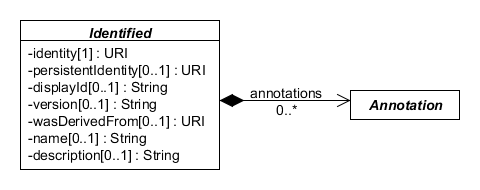
\includegraphics[scale=0.6]{uml/identified}
\caption[]{Diagram of the \sbol{Identified} abstract class and its associated properties}
\label{uml:identified}
\end{center}
\end{figure}

\subsubsection*{The \sbolheading{identity} property}
\label{sec:identity}
The \sbol{identity} property is REQUIRED by all \sbol{Identified} objects and has a data type of \sbol{URI}. A given \sbol{Identified} object's \sbol{identity} \sbol{URI} MUST be globally unique among all other \sbol{identity} \sbol{URI}s. It is also highly RECOMMENDED that the \sbol{URI} structure follows the recommended best practices for compliant \sbol{URI}s specified in \ref{sec:compliant}.

Although most SBOL properties are defined by SBOL and serialized with its namespace, the \sbol{identity} property is defined by the analogous RDF \external{about} property and is serialized with the RDF namespace as follows:

\url{http://www.w3.org/1999/02/22-rdf-syntax-ns\#about}.

The use of \external{about} is expressly for the purpose of making SBOL compliant with pre-existing standards: when you see \external{about} in an SBOL document, you SHOULD interpret it as meaning \sbol{identity}.

\subsubsection*{The \sbolheading{persistentIdentity} property}
\label{sec:persistentIdentity}
The \sbol{persistentIdentity} property is OPTIONAL and has a data type of \sbol{URI}. This \sbol{URI} serves to uniquely refer to a set of SBOL objects \twozeroone{of the same class} that are different versions of each other.

An \sbol{Identified} object MUST be referred to using either its \sbol{identity} \sbol{URI} or its \sbol{persistentIdentity} \sbol{URI}.

\subsubsection*{The \sbolheading{displayId} property}
\label{sec:displayId}
The \sbol{displayId} property is an OPTIONAL identifier with a data type of \sbol{String}. This property is intended to be an intermediate between \sbol{name} and \sbol{identity} that is machine-readable, but more human-readable than the full \sbol{URI} of an \sbol{identity}.

If the \sbol{displayId} property is used, then its \sbol{String} value \twozeroone{\st{SHOULD be locally unique (global uniqueness is not necessary) and}} MUST be composed of only alphanumeric or underscore characters and MUST NOT begin with a digit.

% compliant with the type \external{http://www.w3.org/TR/xmlschema-2/\#NCName}, except that it MUST not include the characters "-" and ".".

\subsubsection*{The \sbolheading{version} property}
\label{sec:version}

The \sbol{version} property is OPTIONAL and has a data type of \sbol{String}. This property can be used to compare two SBOL objects with the same \sbol{persistentIdentity}.

If the \sbol{version} property is used, then it is RECOMMENDED that version numbering follow the conventions of semantic versioning (\url{http://semver.org/}), particularly as implemented by Maven (\url{http://maven.apache.org/}).
This convention represents versions as sequences of numbers and qualifiers that are separated by the characters ``{\tt .}'' and ``{\tt -}'' and are compared in lexicographical order (for example, 1 < 1.3.1 < 2.0-beta).
For a full explanation, see the linked resources.

\subsubsection*{The \sbolheading{wasDerivedFrom} property}
\label{sec:wasDerivedFrom}

The \sbol{wasDerivedFrom} property is OPTIONAL and has a data type of \sbol{URI}. An SBOL object with this property refers to another SBOL object or non-SBOL resource from which this object was derived.

\twozeroone{The \sbol{wasDerivedFrom} property of a \sbol{TopLevel} SBOL object is subject to the following rules.}
If the \sbol{wasDerivedFrom} property of an SBOL object $A$ that refers to an SBOL object $B$ has an identical \sbol{persistentIdentity}, and both $A$ and $B$ have a \sbol{version}, then the \sbol{version} of $B$ MUST precede that of $A$.
In addition, an SBOL object MUST NOT refer to itself via its own \sbol{wasDerivedFrom} property or form a cyclical chain of references via its \sbol{wasDerivedFrom} property and those of other SBOL objects. For example, the reference chain ``$A$ was derived from $B$ and $B$ was derived from $A$'' is cyclical.

\subsubsection*{The \sbolheading{name} property}
\label{sec:name}

The \sbol{name} property is OPTIONAL and has a data type of \sbol{String}. This property is intended to be displayed to a human when visualizing an \sbol{Identified} object.

If an \sbol{Identified} object lacks a name, then software tools SHOULD instead display the object's \sbol{displayId} or \sbol{identity}.
It is RECOMMENDED that software tools give users the ability to switch perspectives between \sbol{name} properties that are human-readable and \sbol{displayId} properties that are less human-readable, but are more likely to be unique.

\subsubsection*{The \sbolheading{description} property}
\label{sec:description}

The \sbol{description} property is OPTIONAL and has a data type of \sbol{String}. This property is intended to contain a more thorough text description of an \sbol{Identified} object.

\subsubsection*{The \sbolheading{annotations} property}
\label{sec:annotations}

The \sbol{annotations} property is OPTIONAL and MAY specify a set of \sbol{Annotation} objects that are contained by the \sbol{Identified} object. The \sbol{Annotation} class is described in more detail in Section~\ref{sec:Annotation}.

\subsubsection*{Serialization}

No complete serialization is defined for \sbol{Identified}, since this
class is only used indirectly through its child classes.  Any such
child class, however, has the following form for serializing
properties inherited from \sbol{Identified}, where CLASS\_NAME is
replaced by the name of the class:

\lstsetsbol
\begin{lstlisting}
<?xml version="1.0" ?>
<rdf:RDF xmlns:pr="http://partsregistry.org" xmlns:rdf="http://www.w3.org/1999/02/22-rdf-syntax-ns#" xmlns:dcterms="http://purl.org/dc/terms/" xmlns:prov="http://www.w3.org/ns/prov#" xmlns:sbol="http://sbols.org/v2#">
  <sbol:CLASS_NAME rdf:about="...">
    [\emph{zero or one}] <sbol:persistentIdentity rdf:resource="..."/> [\emph{element}]
    [\emph{zero or one}] <sbol:displayId>...</sbol:displayId> [\emph{element}]
    [\emph{zero or one}] <sbol:version>...</sbol:version> [\emph{element}]
    [\emph{zero or one}] <prov:wasDerivedFrom rdf:resource="..."/> [\emph{element}]
    [\emph{zero or one}] <dcterms:title>...</dcterms:title> [\emph{element}]
    [\emph{zero or one}] <dcterms:description>...</dcterms:description> [\emph{element}]
               ...
  </sbol:CLASS_NAME>
  ...
</rdf:RDF>
\end{lstlisting}

Note that several of the properties are not in the \external{sbol}
namespace, but are mapped to standardized terms defined elsewhere:
\begin{itemize}
\item \sbol{identity} is serialized as \external{rdf:about}
\item \sbol{wasDerivedFrom} is serialized as \external{prov:wasDerivedFrom}
\item \sbol{name} is serialized as \external{dcterms:title}
\item \sbol{description} is serialized as \external{dcterms:description}
\end{itemize}

% \subsection{Documented}
% \label{sec:Documented}
% The \sbol{Documented} abstract class is inherited by the classes of SBOL objects that can contain human-readable properties, such as name and description. This class extends \sbol{Identified} with two additional data properties: \sbol{name}, and \sbol{description} (\ref{uml:documented}).

% \begin{figure}[ht]
% \begin{center}
% 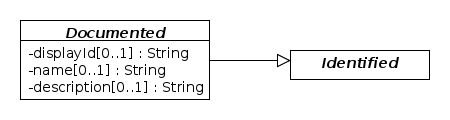
\includegraphics[scale=0.6]{uml/documented}
% \caption[]{The \sbol{Documented} abstract class.}
% \label{uml:documented}
% \end{center}
% \end{figure}

% \subsubsection*{Serialization}

% No complete serialization is defined for \sbol{Documented}, since this
% class is only used indirectly through its child classes.  Any such
% child class, however, has the following form for serializing
% properties inherited from \sbol{Documented}, where CLASS\_NAME is
% replaced by the name of the class:

\subsection {TopLevel}
\label{sec:TopLevel}
\sbol{TopLevel} is an abstract class that is extended by any \sbol{Identified} class that can be found at the top level of an SBOL document or file. In other words, \sbol{TopLevel} objects are not nested inside any other object via a composite aggregation or black diamond arrow association property. Instead of nesting, composite \sbol{TopLevel} objects refer to subordinate \sbol{TopLevel} objects by their \sbol{URI}s using shared aggregation or white diamond arrow association properties. The \sbol{TopLevel} classes defined in this specification are \sbol{Sequence}, \sbol{ComponentDefinition}, \sbol{Model}, \sbol{ModuleDefinition},  \sbol{Collection}, and \sbol{GenericTopLevel} (\ref{uml:toplevel}).

\begin{figure}[ht]
\begin{center}
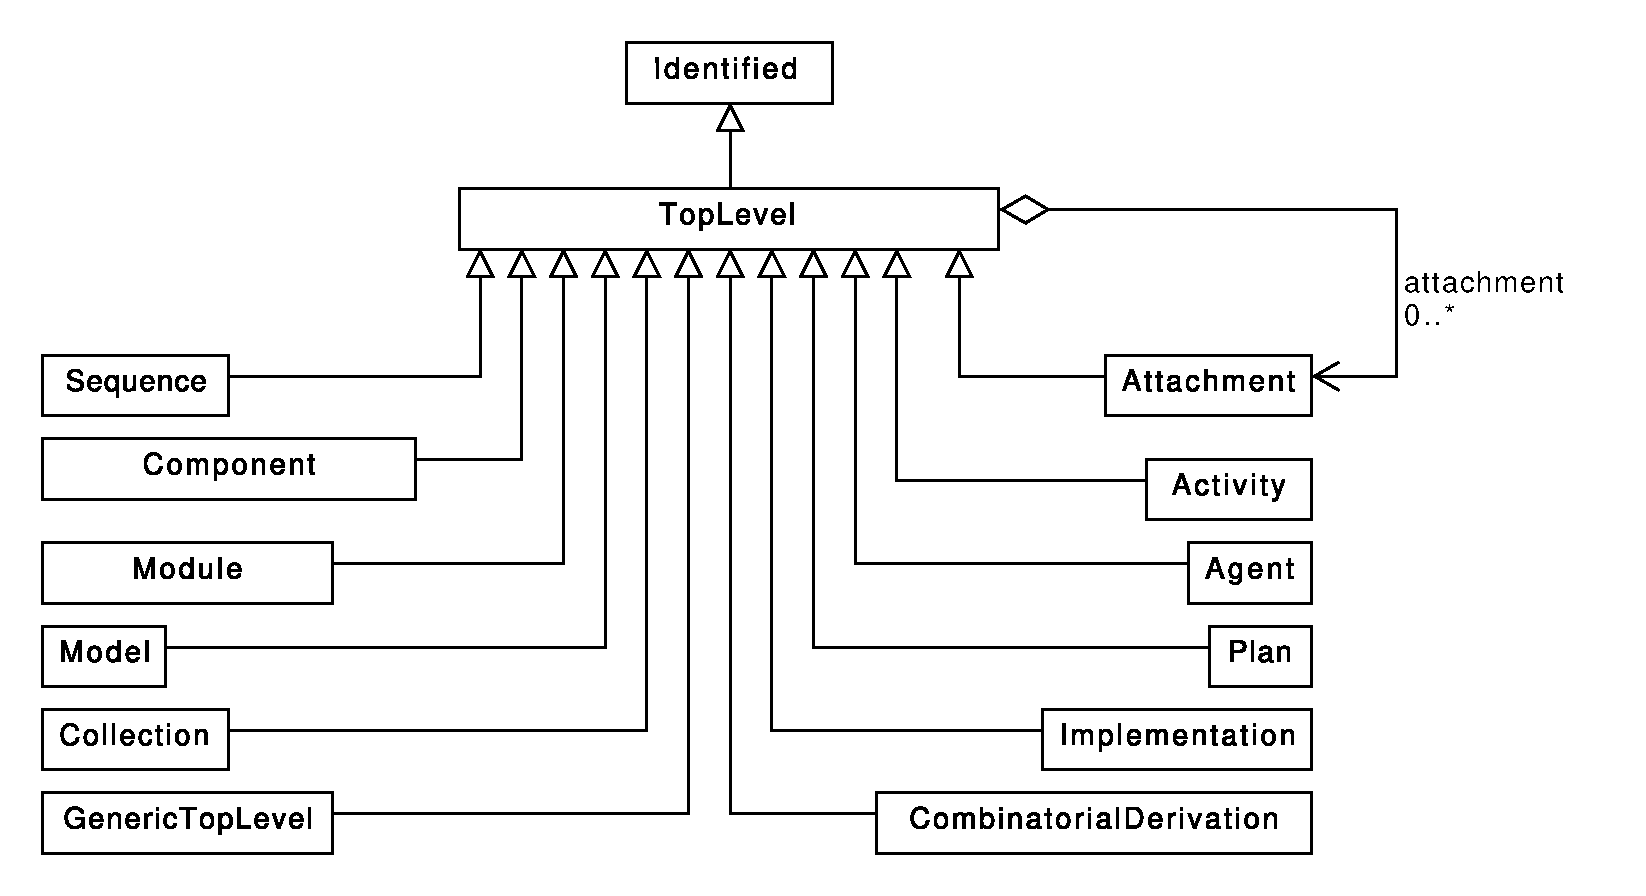
\includegraphics[width=\textwidth]{uml/toplevel}
\caption[]{Classes that inherit from the \sbol{TopLevel} abstract class.}
\label{uml:toplevel}
\end{center}
\end{figure}

\subsubsection*{Serialization}

No serialization is defined for \sbol{TopLevel}, since this class has no properties of its own and is only used indirectly through its child classes.  All \sbol{TopLevel} classes are serialized one level beneath the RDF document root.


\subsection{Sequence}
\label{sec:Sequence}
The purpose of the \sbol{Sequence} class is to represent the primary structure of a \sbol{ComponentDefinition} object and the manner in which it is encoded. This representation is accomplished  by means of the \sbol{elements} property and \sbol{encoding} property (\ref{uml:sequence}).

\begin{figure}[ht]
\begin{center}
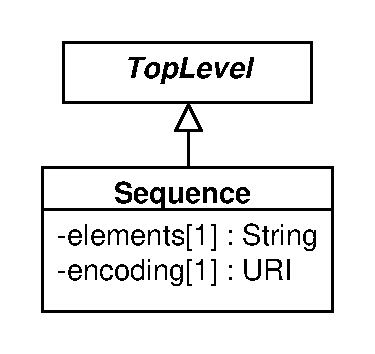
\includegraphics[scale=0.6]{uml/sequence}
\caption[]{Diagram of the \sbol{Sequence} class and its associated properties.}
\label{uml:sequence}
\end{center}
\end{figure}


\subsubsection*{The \sbolheading{elements} property}
\label{sec:elements}
The \sbol{elements} property is a REQUIRED \sbol{String} of characters that represents the constituents of a biological or chemical molecule. For example, these characters could represent the nucleotide bases of a molecule of DNA, the amino acid residues of a protein, or the atoms and chemical bonds of a small molecule.

\subsubsection*{The \sbolheading{encoding} property}
\label{sec:encoding}
The \sbol{encoding} property is REQUIRED and has a data type of \sbol{URI}. This property MUST indicate how the \sbol{elements} property of a \sbol{Sequence} MUST be formed and interpreted.

For example, the \sbol{elements} property of a \sbol{Sequence} with an \external{IUPAC DNA} encoding property MUST contain characters that represent nucleotide bases, such as {\tt a}, {\tt t}, {\tt c}, and {\tt g}. The \sbol{elements} property of a \sbol{Sequence} with a \external{Simplified Molecular-Input Line-Entry System (SMILES)} encoding, on the other hand, MUST contain characters that represent atoms and chemical bonds, such as {\tt C}, {\tt N}, {\tt O}, and {\tt =}.

\ref{tbl:sequence_encodings} provides a list of possible \sbol{URI} values for the \sbol{encoding} property. The terms in \ref{tbl:sequence_encodings} are organized by the type of \sbol{ComponentDefinition} (see \ref{tbl:componentdefinition_types}) that typically refer to a \sbol{Sequence} with such an \sbol{encoding}. \twozeroone{It is RECOMMENDED that the encoding property of a Sequence contains a URI from \ref{tbl:sequence_encodings}.} When the \sbol{encoding} of a \sbol{Sequence} is well described by one of the \sbol{URI}s in \ref{tbl:sequence_encodings}, it MUST contain that \sbol{URI}.

%A Summary of letters for nucleic acids and aminoacids
\begin{table}[ht]
  \begin{edtable}{tabular}{lll}
    \toprule
     \textbf{Encoding} & \textbf{URI} & \textbf{ComponentDefinition Type} \\
    \midrule
     IUPAC DNA, RNA & \url{http://www.chem.qmul.ac.uk/iubmb/misc/naseq.html} & DNA, RNA \\
    IUPAC Protein & \url{http://www.chem.qmul.ac.uk/iupac/AminoAcid/} & Protein\\
   SMILES & \url{http://www.opensmiles.org/opensmiles.html} & SmallMolecule \\
    \bottomrule
  \end{edtable}
  \caption{\sbol{URI}s for specifying the \sbol{encoding} property of a \sbol{Sequence}, organized by the type of \sbol{ComponentDefinition} (see \ref{tbl:componentdefinition_types}) that typically refer to a \sbol{Sequence} with such an \sbol{encoding}.}
  \label{tbl:sequence_encodings}
\end{table}

\subsubsection*{Serialization}
The serialization of a \sbol{Sequence} MUST have the following form:
\lstsetsbol
\begin{lstlisting}
<sbol:Sequence rdf:about="...">
  ... [\emph{properties inherited from identified}] ...
  [\emph{one}] <sbol:elements>...</sbol:elements> [\emph{element}]
  [\emph{one}] <sbol:encoding rdf:resource="..."/> [\emph{element}]
</sbol:Sequence>
\end{lstlisting}

The example below shows the serialization of the \sbol{Sequence} for a promoter. The nucleotide bases of the \sbol{Sequence} are serialized as the \sbol{String} value of its \sbol{elements} property, while its \external{IUPAC DNA} encoding is serialized as the \sbol{URI} value of its  \sbol{encoding} property.

\lstsetsbol
\begin{lstlisting}
<?xml version="1.0" ?>
<rdf:RDF xmlns:rdf="http://www.w3.org/1999/02/22-rdf-syntax-ns#" xmlns:dcterms="http://purl.org/dc/terms/" xmlns:prov="http://www.w3.org/ns/prov#" xmlns:sbol="http://sbols.org/v2#">
  <sbol:Sequence rdf:about="http://partsregistry.org/seq/BBa_J23119">
    <sbol:persistentIdentity rdf:resource="http://partsregistry.org/seq/BBa_J23119"/>
    <sbol:displayId>BBa_J23119</sbol:displayId>
    <prov:wasDerivedFrom rdf:resource="http://parts.igem.org/Part:BBa_J23119:Design"/>
    <sbol:elements>ttgacagctagctcagtcctaggtataatgctagc</sbol:elements>
    <sbol:encoding rdf:resource="http://www.chem.qmul.ac.uk/iubmb/misc/naseq.html"/>
  </sbol:Sequence>
</rdf:RDF>
\end{lstlisting}


\subsection{ComponentDefinition}
\label{sec:ComponentDefinition}

The \sbol{ComponentDefinition} class represents the structural entities of a biological design. The primary usage of this class is to represent structural entities with designed sequences, such as DNA, RNA, and proteins, but it can also be used to represent any other entity that is part of a design, such as small molecules, molecular complexes, and light.

As shown in \ref{uml:component_definition}, the \sbol{ComponentDefinition} class describes a structural design entity using the following properties: \sbolmult{types:CD}{types}, \sbolmult{roles:CD}{roles}, and \sbol{sequences}. In addition, this class has properties for describing and organizing the substructure of said design entity, including \sbol{components}, \sbol{sequenceAnnotations}, and \sbol{sequenceConstraints}.

\begin{figure}[ht]
\begin{center}
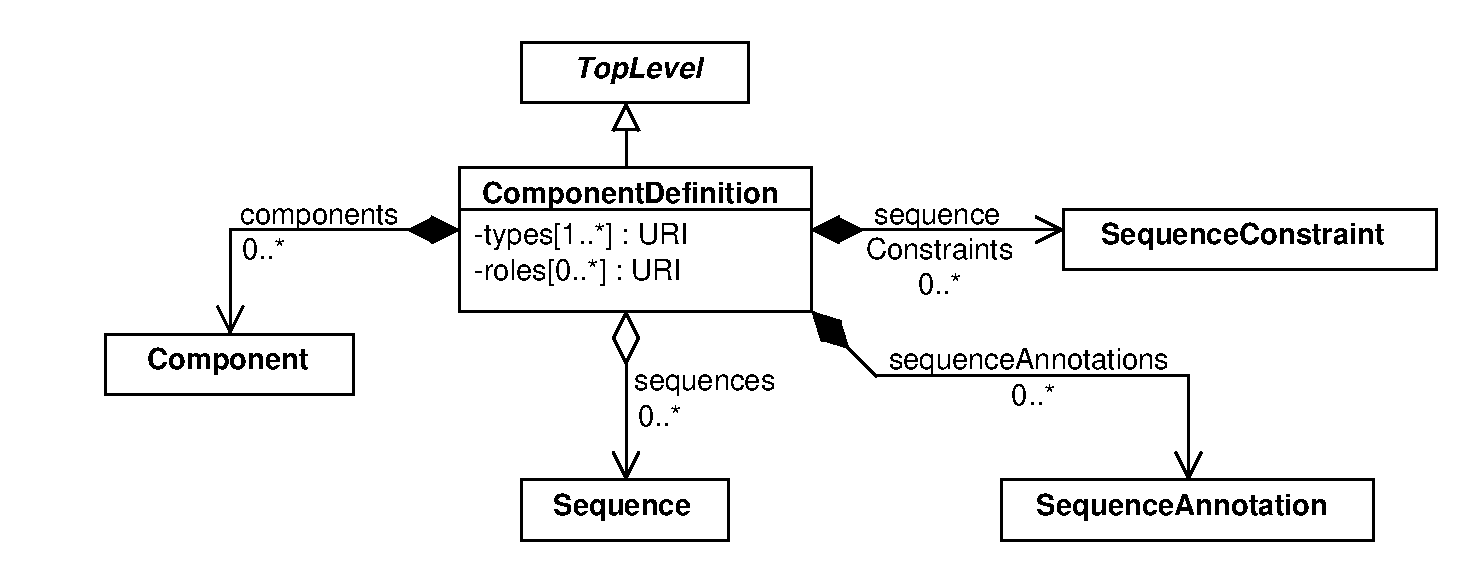
\includegraphics[width=0.95\textwidth]{uml/component_definition}
\caption[]{Diagram of the \sbol{ComponentDefinition} class and its associated properties.}
\label{uml:component_definition}
\end{center}
\end{figure}

\subsubsection*{The \sbolheading{types} property}
\label{sec:types:CD}

The \sbolmult{types:CD}{types} property is a REQUIRED set of \sbol{URI}s that specifies the category of biochemical or physical entity (for example DNA, protein, or small molecule) that a \sbol{ComponentDefinition} object abstracts for the purpose of engineering design.

The \sbolmult{types:CD}{types} property of every \sbol{ComponentDefinition} MUST contain one or more \sbol{URI}s that MUST identify terms from appropriate ontologies, such as the BioPAX ontology or the ontology of Chemical Entities of Biological Interest (ChEBI).
\ref{tbl:componentdefinition_types} provides a list of possible ontology terms for the \sbolmult{types:CD}{types} property and their \sbol{URI}s.
In order to maximize the compatibility of designs, \twozeroone{the \sbolmult{types:CD}{types} property of a \sbol{ComponentDefinition} SHOULD contain a \sbol{URI} from \ref{tbl:componentdefinition_types}, and} any \sbol{ComponentDefinition} that can be well-described by one of the terms in \ref{tbl:componentdefinition_types} MUST use the \sbol{URI} for that term as one of its \sbolmult{types:CD}{types}.
Finally, if the \sbolmult{types:CD}{types} property contains multiple \sbol{URI}s, then they MUST identify non-conflicting terms (otherwise, it might not be clear how to interpret them). For example, the BioPAX terms provided by \ref{tbl:componentdefinition_types} would conflict because they specify classes of biochemical entities with different molecular structures.

\begin{table}[ht]
  \begin{edtable}{tabular}{ll}
    \toprule
    \textbf{ComponentDefinition Type} & \textbf{URI for BioPAX Term} \\
    \midrule
    DNA  & \url{http://www.biopax.org/release/biopax-level3.owl#DnaRegion}\\
    RNA  & \url{http://www.biopax.org/release/biopax-level3.owl#RnaRegion}\\
    Protein  & \url{http://www.biopax.org/release/biopax-level3.owl#Protein}\\
    Small Molecule  & \url{http://www.biopax.org/release/biopax-level3.owl#SmallMolecule}\\
    Complex  & \url{http://www.biopax.org/release/biopax-level3.owl#Complex}\\
    \bottomrule
  \end{edtable}
  \caption{BioPAX terms to specify the \sbolmult{types:CD}{types} property of a \sbol{ComponentDefinition}.}
 \label{tbl:componentdefinition_types}
\end{table}

\subsubsection*{The \sbolheading{roles} property}
\label{sec:roles:CD}

The \sbolmult{roles:CD}{roles} property is an OPTIONAL set of \sbol{URI}s that clarifies the potential function of the entity represented by a \sbol{ComponentDefinition} in a biochemical or physical context.

The \sbolmult{roles:CD}{roles} property of a \sbol{ComponentDefinition} MAY contain one or more \sbol{URI}s that MUST identify terms from ontologies that are consistent with the \sbolmult{types:CD}{types} property of the \sbol{ComponentDefinition}.
For example, the \sbolmult{roles:CD}{roles} property of a DNA or RNA \sbol{ComponentDefinition} could contain URIs identifying terms from the Sequence Ontology (SO). \twozeroone{As a best practice, a DNA or RNA \sbol{ComponentDefinition} SHOULD contain exactly one \sbol{URI} that refers to a term from the sequence feature branch of the SO.}
\ref{tbl:componentdefinition_roles} contains a list of possible ontology terms for the \sbolmult{roles:CD}{roles} property and their \sbol{URI}s. These terms are organized by the type of \sbol{ComponentDefinition} to which they SHOULD apply (see \ref{tbl:componentdefinition_types}). Any \sbol{ComponentDefinition} that can be well-described by one of the terms in \ref{tbl:componentdefinition_roles} MUST use the \sbol{URI} for that term as one of its \sbolmult{roles:CD}{roles}.


\begin{table}[ht]
  \begin{edtable}{tabular}{lll}
    \toprule
    \textbf{ComponentDefinition Role} & \textbf{URI for Ontology Term} & \textbf{ComponentDefinition Type} \\
    \midrule
   Promoter & \url{http://identifiers.org/so/SO:0000167} & DNA \\
   RBS & \url{http://identifiers.org/so/SO:0000139} & DNA \\
      CDS & \url{http://identifiers.org/so/SO:0000316} & DNA \\
      Terminator & \url{http://identifiers.org/so/SO:0000141} & DNA \\
      Gene & \url{http://identifiers.org/so/SO:0000704} & DNA \\
      Operator & \url{http://identifiers.org/so/SO:0000057} & DNA \\
      Engineered Gene & \url{http://identifiers.org/so/SO:0000280} & DNA \\
      mRNA & \url{http://identifiers.org/so/SO:0000234} & RNA \\
      Effector & \url{http://identifiers.org/chebi/CHEBI:35224} & Small Molecule \\
    \bottomrule
  \end{edtable}
  \caption{Ontology terms to specify the \sbolmult{roles:CD}{roles} property of a \sbol{ComponentDefinition}, organized by the type of \sbol{ComponentDefinition} to which they are intended to apply (see \ref{tbl:componentdefinition_types}).}
  \label{tbl:componentdefinition_roles}
\end{table}

\subsubsection*{The \sbolheading{sequences} property}
\label{sec:sequences}
The \sbol{sequences} property is OPTIONAL and MAY include a set of \sbol{URI}s that refer to \sbol{Sequence} objects. These objects define the primary structure of the \sbol{ComponentDefinition}.

Many \sbol{ComponentDefinition} objects will refer to precisely one \sbol{Sequence} object.
For certain use cases, however, it can be appropriate to refer to multiple \sbol{Sequence} objects.
For example, a user might wish to provide two different representations of the structure of a DNA \sbol{ComponentDefinition}, one that represents its structure at the level of nucleotide bases and one that represents its structure at the level of atoms and bonds.

If a \sbol{ComponentDefinition} refers to more than one \sbol{Sequence} object, then these objects MUST be consistent with each other, such that well-defined mappings exist between their \sbol{elements} properties in accordance with their \sbol{encoding} properties. Furthermore, these objects MUST NOT have conflicting \sbol{encoding} properties. For example, the \external{IUPAC} \sbol{encoding} properties provided by \ref{tbl:sequence_encodings} conflict with each other because they do not specify how to encode the same class of biochemical entity. The \external{SMILES} \sbol{encoding}, however, does not conflict with them because it specifies how to encode biochemical entities in general, which includes DNA, RNA, and proteins. If a \sbol{ComponentDefinition} refers to more than one \sbol{Sequence} with the same \sbol{encoding}, then the \sbol{elements} of these \sbol{Sequence} objects SHOULD have equal lengths. These requirements and best practices are intended to make it easier for software tools to locate any regions specified by the \sbol{SequenceAnnotation} objects of a \sbol{ComponentDefinition} on its associated \sbol{Sequence} objects, as well as validate whether its \sbol{Sequence} objects are consistent with those associated with any \sbol{ComponentDefinition} objects that it composes via its \sbol{Component} objects.

Finally, if a \sbol{ComponentDefinition} refers to one or more \sbol{Sequence} objects and its \sbolmult{types:CD}{types} property refers to a term from \ref{tbl:componentdefinition_types}, then one of these \sbol{Sequence} objects MUST have the \sbol{encoding} that is cross-listed with this term in \ref{tbl:sequence_encodings}.
Conversely, if a \sbol{ComponentDefinition} refers to a \sbol{Sequence} with an \sbol{encoding} from \ref{tbl:sequence_encodings}, then its \sbolmult{types:CD}{types} property MUST refer to the term from \ref{tbl:componentdefinition_types} that is cross-listed with this \sbol{encoding} in \ref{tbl:sequence_encodings}.
For example, if the \sbolmult{types:CD}{types} property of a \sbol{ComponentDefinition} refers to the BioPAX term for DNA, then one of the \sbol{Sequence} objects to which it refers (if any) MUST have an \external{IUPAC DNA} \sbol{encoding}, and if a \sbol{ComponentDefinition} refers to a \sbol{Sequence} with an \external{IUPAC DNA} \sbol{encoding}, then its \sbolmult{types:CD}{types} property MUST refer to the BioPAX term for DNA. These requirements are meant to provide for some degree of consistency between the \sbolmult{types:CD}{types} property of a \sbol{ComponentDefinition} and the \sbol{encoding} properties of the \sbol{Sequence} objects to which the \sbol{ComponentDefinition} refers.

\subsubsection*{The \sbolheading{components} property}
\label{sec:components}

The \sbol{components} property is OPTIONAL and MAY specify a set of \sbol{Component} objects that are contained by the \sbol{ComponentDefinition}. The set of relations between \sbol{Component} and \sbol{ComponentDefinition} objects is strictly acyclic (see \ref{sec:ComponentInstance}).

While the \sbol{ComponentDefinition} class is analogous to a blueprint or specification sheet for a biological part, the \sbol{Component} class represents the specific occurrence of a part within a design.
Hence, this class allows a biological design to include multiple instances of a particular part (defined by reference to the same \sbol{ComponentDefinition}). For example, the \sbol{ComponentDefinition} of a polycistronic gene could contain two \sbol{Component} objects that refer to the same \sbol{ComponentDefinition} of a CDS.

The \sbol{components} properties of \sbol{ComponentDefinition} objects can be used to construct a hierarchy of \sbol{Component} and \sbol{ComponentDefinition} objects. If a \sbol{ComponentDefinition} in such a hierarchy refers to one or more \sbol{Sequence} objects, and there exist \sbol{ComponentDefinition} objects lower in the hierarchy that refer to \sbol{Sequence} objects with the same \sbol{encoding}, then the \sbol{elements} properties of these \sbol{Sequence} objects SHOULD be consistent with each other, such that well-defined mappings exist from the ``lower level'' \sbol{elements} to the ``higher level'' \sbol{elements} in accordance with their shared \sbol{encoding} properties. This mapping is also subject to any restrictions on the positions of the \sbol{Component} objects in the hierarchy that are imposed by the \sbol{SequenceAnnotation} or \sbol{SequenceConstraint} objects contained by the \sbol{ComponentDefinition} objects in the hierarchy.

A DNA \sbol{ComponentDefinition}, for example, could refer to a \sbol{Sequence} with an \external{IUPAC DNA} \sbol{encoding} and an \sbol{elements} \external{String} of ``{\tt gattaca}.'' In turn, this \sbol{ComponentDefinition} could contain a \sbol{Component} that refers to a ``lower level''  \sbol{ComponentDefinition} that also refers to a \sbol{Sequence} with an \external{IUPAC DNA} \sbol{encoding}. Consequently, a consistent \sbol{elements} \external{String} of this ``lower level'' \sbol{Sequence} could be ``{\tt gatta}," or perhaps ``{\tt tgta}'' if the \sbol{Component} is positioned by a \sbol{SequenceAnnotation} that contains a \sbol{Location}  with an \sbol{orientation} of ``reverse complement'' (see \ref{sec:Location}).

% If the \sbol{ComponentDefinition} refers to a \sbol{Sequence} with an \external{IUPAC} \sbol{encoding} from \ref{tbl:sequence_encodings}, then each \sbol{Component} in its \sbol{components} property MUST refer to a \sbol{ComponentDefinition} that refers to a \sbol{Sequence} with the same \sbol{encoding}.
% In addition, it MUST be possible to align the \sbol{elements} of the latter \sbol{Sequence} objects to the \sbol{elements} of the \sbol{ComponentDefinition}'s \sbol{Sequence}, subject to any restrictions imposed by the \sbol{SequenceAnnotation} and \sbol{SequenceConstraint} objects that refer to the contents of the \sbol{components} property.
% A DNA \sbol{ComponentDefinition}, for example, could refer to a \sbol{Sequence} that has an \external{IUPAC DNA} \sbol{encoding} and an \sbol{elements} \external{String} of ``{\tt gattaca}.'' In this case, any \sbol{Component} contained by this \sbol{ComponentDefinition} would itself need to have a \sbol{ComponentDefinition} that refers to a \sbol{Sequence} that has an \external{IUPAC DNA} \sbol{encoding} and an \sbol{elements} \external{String} that can be aligned with ``{\tt gattaca},'' such as ``{\tt gatta}," or perhaps ``{\tt tgta}'' in the case of a \sbol{Component} that is positioned by a \sbol{SequenceAnnotation} with a \sbol{Location} \sbol{orientation} of ``reverse complement'' (see \ref{sec:Location}).

% Furthermore, this \sbol{Sequence} MUST have the same \external{IUPAC} \sbol{encoding} as a \sbol{Sequence} of the parent \sbol{ComponentDefinition} that contains the \sbol{SequenceAnnotation}.

\subsubsection*{The \sbolheading{sequenceAnnotations} property}
\label{sec:sequenceAnnotations}

The \sbol{sequenceAnnotations} property is OPTIONAL and MAY contain a set of \sbol{SequenceAnnotation} objects. Each \sbol{SequenceAnnotation} specifies and describes a potentially discontiguous region on the \sbol{Sequence} objects referred to by the \sbol{ComponentDefinition}.

In addition, each \sbol{SequenceAnnotation} can  position a \sbol{Component} of the \sbol{ComponentDefinition} at the region specified by its \sbol{Location} objects (see \ref{sec:Location}). The \sbol{sequenceAnnotations} property MUST NOT contain two or more \sbol{SequenceAnnotation} objects that refer to the same \sbol{Component} in this way.

Finally, as a best practice, if a \sbol{ComponentDefinition} refers to a \sbol{Sequence} with an \external{IUPAC} \sbol{encoding} from \ref{tbl:sequence_encodings}, then each of its \sbol{SequenceAnnotation} objects that contains a \sbol{Range} or \sbol{Cut} SHOULD specify a region on the \sbol{elements} of this \sbol{Sequence}.
For example, the \sbol{ComponentDefinition} of a eukaryotic gene could refer to a \sbol{Sequence} with an \external{IUPAC DNA} \sbol{encoding}. In order to specify the discontiguous region occupied by its CDS, this gene \sbol{ComponentDefinition} would need a \sbol{SequenceAnnotation} that contains one or more \sbol{Range} objects, each one specifying \sbol{start} and \sbol{end} positions that correspond to indices of the \sbol{elements} of its DNA \sbol{Sequence}.

\subsubsection*{The \sbolheading{sequenceConstraints} property}
\label{sec:sequenceConstraints}

The \sbol{sequenceConstraints} property is OPTIONAL and MAY contain a set of \sbol{SequenceConstraint} objects. These objects describe any restrictions on the relative, sequence-based positions and/or orientations of the \sbol{Component} objects contained by the \sbol{ComponentDefinition}.
For example, the \sbol{ComponentDefinition} of a gene might specify that the position of its promoter \sbol{Component} precedes that of its CDS \sbol{Component}. This is particularly useful when a \sbol{ComponentDefinition} lacks a \sbol{Sequence} and therefore cannot specify the precise, sequence-based positions of its \sbol{Component} objects using \sbol{SequenceAnnotation} objects.

\subsubsection*{Serialization}
The serialization of a \sbol{ComponentDefinition} MUST have the form below.
The \sbol{components},  \sbol{sequenceConstraints},  \sbol{sequenceAnnotations}, and \sbol{sequences} properties of a \sbol{ComponentDefinition} contain or reference objects belonging to the appropriate SBOL classes as their values, while the \sbolmult{types:CD}{types} and \sbolmult{roles:CD}{roles} properties contain \sbol{URI}s that identify ontology terms as their values.

As shown below, each of these objects and \sbol{URI}s are serialized as part of an implicit set of SBOL properties with singular rather then plural names.
In particular, each object is serialized as an RDF/XML node nested within a property, while each \sbol{URI} (except the \sbol{identity}) is serialized as an \external{rdf:resource} on a property.

\lstsetsbol
\begin{lstlisting}
<sbol:ComponentDefinition rdf:about="...">
  ... [\emph{properties inherited from identified}] ...
  [\emph{zero or more}]  <sbol:sequence rdf:resource="..."/> [\emph{element}]
  [\emph{one or more}]   <sbol:type rdf:resource="..."/> [\emph{elements}]
  [\emph{zero or more}]  <sbol:role rdf:resource="..."/> [\emph{elements}]
  [\emph{zero or more}]  <sbol:component>
                 <sbol:Component rdf:about="...">...</sbol:Component>
               </sbol:component> [\emph{elements}]
  [\emph{zero or more}] <sbol:sequenceAnnotation>
                 <sbol:SequenceAnnotation rdf:about="...">...</sbol:SequenceAnnotation>
               </sbol:sequenceAnnotation> [\emph{elements}]
  [\emph{zero or more}] <sbol:sequenceConstraint>
                 <sbol:SequenceConstraint rdf:about="...">...</sbol:SequenceConstraint>
               </sbol:sequenceConstraint> [\emph{elements}]
</sbol:ComponentDefinition>
\end{lstlisting}


The example below shows the serialization for the \sbol{ComponentDefinition} of a promoter. The BioPAX term \external{DnaRegion} and the ChEBI term \external{CHEBI:4705} (\external{double-stranded DNA}) are used to indicate that the type of biological entity represented by this \sbol{ComponentDefinition} is DNA. Its role is specified using the SO terms \external{SO:0000167} (\external{promoter}) and the more specific \external{SO:0000613} (\external{bacterial\_RNApol\_promoter}).

\lstsetsbol
\begin{lstlisting}
<?xml version="1.0" ?>
<rdf:RDF xmlns:rdf="http://www.w3.org/1999/02/22-rdf-syntax-ns#" xmlns:dcterms="http://purl.org/dc/terms/" xmlns:prov="http://www.w3.org/ns/prov#" xmlns:sbol="http://sbols.org/v2#">
  <sbol:ComponentDefinition rdf:about="http://partsregistry.org/cd/BBa_J23119">
    <sbol:persistentIdentity rdf:resource="http://partsregistry.org/cd/BBa_J23119"/>
    <sbol:displayId>BBa_J23119</sbol:displayId>
    <prov:wasDerivedFrom rdf:resource="http://partsregistry.org/Part:BBa_J23119"/>
    <dcterms:title>J23119 promoter</dcterms:title>
    <dcterms:description>Constitutive promoter</dcterms:description>
    <sbol:type rdf:resource="http://identifiers.org/chebi/CHEBI:4705"/>
    <sbol:type rdf:resource="http://www.biopax.org/release/biopax-level3.owl#DnaRegion"/>
    <sbol:role rdf:resource="http://identifiers.org/so/SO:0000167"/>
    <sbol:role rdf:resource="http://identifiers.org/so/SO:0000613"/>
    <sbol:sequence rdf:resource="http://partsregistry.org/seq/BBa_J23119"/>
  </sbol:ComponentDefinition>
</rdf:RDF>
\end{lstlisting}


\subsubsection{ComponentInstance}
\label{sec:ComponentInstance}

\begin{figure}[ht]
\begin{center}
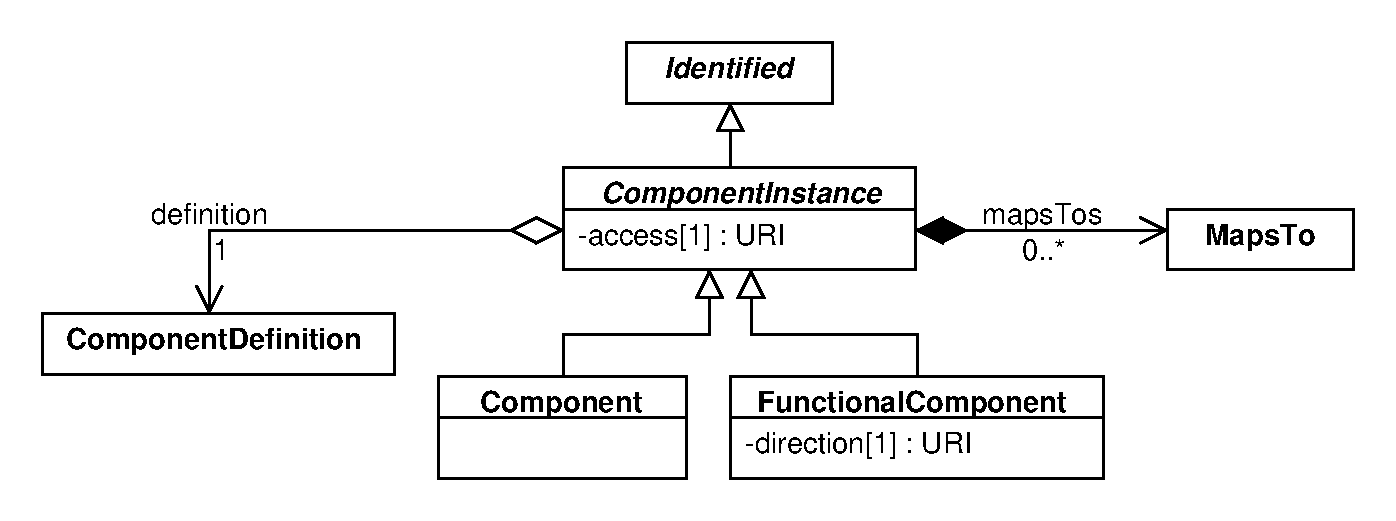
\includegraphics[scale=0.6]{uml/component_instance}
\caption[]{Diagram of the \sbol{ComponentInstance} class and its associated properties.}
\label{uml:component}
\end{center}
\end{figure}

The \sbol{ComponentInstance} abstract class is inherited by SBOL classes that represent the usage or occurrence of a \sbol{ComponentDefinition} within a larger design (that is, another \sbol{ComponentDefinition} or \sbol{ModuleDefinition}). Currently, there are two subclasses of \sbol{ComponentInstance}:
\begin{itemize}
\item The \sbol{Component} class is used to specify the structural usage of a \sbol{ComponentDefinition} inside another \sbol{ComponentDefinition} via the \sbol{components} property.
\item The \sbol{FunctionalComponent} class is used to specify the functional usage of a \sbol{ComponentDefinition} inside a \sbol{ModuleDefinition} via the \sbol{functionalComponents} property. This class is described in \ref{sec:FunctionalComponent}.
\end{itemize}

\paragraph{The \sbolheading{definition} property}
\label{sec:definition:CI}

The \sbolmult{definition:CI}{definition} property is a REQUIRED \sbol{URI} that refers to the \sbol{ComponentDefinition} of the \sbol{ComponentInstance}.
As described in the previous section, this \sbol{ComponentDefinition} effectively provides information about the \sbolmult{types:CD}{types} and \sbolmult{roles:CD}{roles} of the \sbol{ComponentInstance}.

The \sbolmult{definition:CI}{definition} property MUST NOT refer to the same \sbol{ComponentDefinition} as the one that contains the \sbol{ComponentInstance}.
Furthermore, \sbol{ComponentInstance} objects MUST NOT form a cyclical chain of references via their \sbolmult{definition:CI}{definition} properties and the \sbol{ComponentDefinition} objects that contain them.
For example, consider the \sbol{ComponentInstance} objects $A$ and $B$ and the \sbol{ComponentDefinition} objects $X$ and $Y$. The reference chain ``$X$ contains $A$, $A$ is defined by $Y$, $Y$ contains $B$, and $B$ is defined by $X$'' is cyclical.

\paragraph{The \sbolheading{mapsTos} property}\label{sec:mapsTos:CI}

The \sbolmult{mapsTos:CI}{mapsTos} property is OPTIONAL and MAY contain a set of \sbol{MapsTo} objects that refer to and link together \sbol{ComponentInstance} objects (both \sbol{Component} objects and \sbol{FunctionalComponent} objects) within a larger design.

\ref{sec:MapsTo} contains a more detailed description of the \sbol{MapsTo} class.

\paragraph{The \sbolheading{access} property}
\label{sec:access}
\label{sec:public}
\label{sec:private}

The \sbol{access} property is a REQUIRED \sbol{URI} that indicates whether the \sbol{ComponentInstance}
can be referred to remotely by a \sbol{MapsTo} on another \sbol{ComponentInstance} or \sbol{Module} contained by a different parent \sbol{ComponentDefinition} or \sbol{ModuleDefinition} (one that does not contain this \sbol{ComponentInstance}).

\ref{tbl:componentInstance_access} provides a list of REQUIRED \sbol{access} \sbol{URI}s. The value of the \sbol{access} property MUST be one of these \sbol{URI}s.

\begin{table}[ht]
  \begin{edtable}{tabular}{lp{4in}}
    \toprule
    \textbf{Access URI} & \textbf{Description} \\
    \midrule
    \url{http://sbols.org/v2#public}  & The \sbol{ComponentInstance} MAY be referred to by remote \sbol{MapsTo} objects. \\
        \url{http://sbols.org/v2#private}  & The \sbol{ComponentInstance} MUST NOT be referred to by remote \sbol{MapsTo} objects. \\
    \bottomrule
  \end{edtable}
  \caption{REQUIRED \sbol{URI}s for the \sbol{access} property.}
  \label{tbl:componentInstance_access}
\end{table}

In some cases, a designer might want to set the \sbol{access} property of a \sbol{ComponentInstance} such that others cannot map to the \sbol{ComponentInstance} when they reuse its parent \sbol{ComponentDefinition}. For example, a designer who is concerned about retroactivity might set the \sbol{access} of the \sbol{ComponentInstance} to ``private'' in order to prevent its mapping to another \sbol{ComponentInstance} that participates in a new \sbol{Interaction} as part of a composite design.

\paragraph{Serialization}

No serialization is defined for the \sbol{ComponentInstance} class, since this class is only used indirectly through the \sbol{Component} and \sbol{FunctionalComponent} subclasses.

\subsubsection{Component}
\label{sec:Component}
The \sbol{Component} class is used to compose \sbol{ComponentDefinition} objects into a structural hierarchy. For example, the \sbol{ComponentDefinition} of a gene could contain four \sbol{Component} objects: a promoter, RBS, CDS, and terminator. In turn, the \sbol{ComponentDefinition} of the promoter \sbol{Component} could contain \sbol{Component} objects defined as various operator sites.

% All \sbol{Component} objects directly referenced within a \sbol{ComponentDefinition}'s \sbol{SequenceAnnotation} or \sbol{SequenceConstraint} parts MUST be associated with that \sbol{ComponentDefinition} by means of its \sbol{components} property.

\twoonezero{

\paragraph{The \sbolheading{roles} property}\label{sec:roles:C}
\vspace{-7pt}
\-\hspace{0.8cm}[New in 2.1.0; see SEP 004: \url{https://github.com/SynBioDex/SEPs/issues/4}]

The expected purpose and function of a genetic part are described by the
\sbolmult{roles:CD}{roles} property of \sbol{ComponentDefinition}. However, the same building block might be used for a different purpose in an actual design. In other words, purpose and function are sometimes determined by context. 

The \sbolmult{roles:C}{roles} property comprises an OPTIONAL set of zero or more \sbolmult{roles:C}{role} \sbol{URI}s describing the purpose or potential function of this \sbol{Component}'s included sub-\sbol{ComponentDefinition} in the \textit{context} of its parent \sbol{ComponentDefinition}.
If provided, these \sbolmult{roles:C}{role} \sbol{URI}s MUST identify terms from appropriate ontologies. Roles are not restricted to describing biological function; they may annotate a \sbol{Component}'s function in any domain for which an ontology exists.

It is RECOMMENDED that these \sbolmult{roles:C}{role} \sbol{URI}s identify terms that are compatible with the \sbolmult{types:CD}{type} properties of both this \sbol{Component}'s parent \sbol{ComponentDefinition} and its included sub-\sbol{ComponentDefinition}. For example, a \sbolmult{roles:C}{role} of a \sbol{Component} which belongs to a \sbol{ComponentDefinition} of type DNA and includes a sub-\sbol{ComponentDefinition} of type DNA might refer to terms from the Sequence Ontology. A table of recommended ontology terms for \sbolmult{roles:C}{roles} is given in \ref{tbl:componentdefinition_roles}.
}

\twoonezero{
\paragraph{The \sbolheading{roleIntegration} property}\label{sec:roleIntegration:C}
\vspace{-7pt}
\-\hspace{0.8cm}
[New in 2.1.0; see SEP 004: \url{https://github.com/SynBioDex/SEPs/issues/4}]

A \sbolmult{roleIntegration:C}{roleIntegration} specifies the relationship between a \sbol{Component} instance's own set of \sbolmult{roles:C}{roles} and the set of \sbolmult{roles:CD}{roles} on the included sub-\sbol{ComponentDefinition}.

The \sbolmult{roleIntegration:C}{roleIntegration} property has a data type of \sbol{URI}. A \sbol{Component} instance with zero \sbolmult{roles:C}{roles} MAY OPTIONALLY specify a \sbolmult{roleIntegration:C}{roleIntegration}. A \sbol{Component} instance with one or more \sbolmult{roles:C}{roles} MUST specify a \sbolmult{roleIntegration:C}{roleIntegration} from \ref{tbl:component_roleIntegration}.
If zero \sbol{Component} \sbolmult{roles:C}{roles} are given and no \sbol{Component} \sbolmult{roleIntegration:C}{roleIntegration} is given, then \url{http://sbols.org/v2\#mergeRoles} is assumed.
It is RECOMMENDED to specify a set of \sbol{Component} \sbolmult{roles:C}{roles} only if the integrated result set of roles would differ from the set of \sbolmult{roles:CD}{roles} belonging to this \sbol{Component}'s included sub-\sbol{ComponentDefinition}.
}

\clearpage

\twoonezero{
\begin{table}[ht]
  \begin{edtable}{tabular}{lp{4in}}
    \toprule
    \textbf{roleIntegration URI} & \textbf{Description} \\
    \midrule
    \url{http://sbols.org/v2\#overrideRoles} & In the context of this \sbol{Component}, ignore any \sbolmult{roles:CD}{roles} given for the included sub-\sbol{ComponentDefinition}. Instead use only the set of zero or more \sbolmult{roles:C}{roles} given for this \sbol{Component}. \\
    \url{http://sbols.org/v2\#mergeRoles} & Use the union of the two sets: both the set of zero or more \sbolmult{roles:C}{roles} given for this \sbol{Component} as well as the set of zero or more \sbolmult{roles:CD}{roles} given for the included sub-\sbol{ComponentDefinition}. \\
    \bottomrule
  \end{edtable}
  \caption{Each \sbolmult{roleIntegration:C}{roleIntegration} mode is associated with a rule governing how a \sbol{Component}'s roles are to be combined with the included 
sub-\sbol{ComponentDefinition}'s roles.}
  \label{tbl:component_roleIntegration}
\end{table}
}

\paragraph{Serialization}

\twoonezero{The serialization of a \sbol{Component} MUST have the following form:}

\lstsetsbol
\begin{lstlisting}
<sbol:Component rdf:about="...">
  ... [\emph{properties inherited from identified}] ...
  [\emph{one}]          <sbol:access rdf:resource="..."/> [\emph{element}]
  [\emph{one}]          <sbol:definition rdf:resource="..."/> [\emph{element}]
  [\emph{zero or more}] <sbol:mapsTo rdf:resource="..."/> [\emph{elements}]
  [\emph{zero or more}] <sbol:role rdf:resource="..."/> [\emph{elements}]
  [\emph{zero or one}]  <sbol:roleIntegration rdf:resource="..."/> [\emph{element}]
</sbol:Component>
\end{lstlisting}

The example below shows the serialization of a \sbol{Component}
that represents an instance of a promoter:

\lstsetsbol
\begin{lstlisting}
<sbol:Component rdf:about="http://partsregistry.org/cd/BBa_F2620/pLuxR">
  <sbol:persistentIdentity rdf:resource="http://partsregistry.org/cd/BBa_F2620/pLuxR"/>
  <sbol:displayId>pLuxR</sbol:displayId>
  <sbol:access rdf:resource="http://sbols.org/v2#public"/>
  <sbol:definition rdf:resource="http://partsregistry.org/cd/BBa_R0062"/>
</sbol:Component>
\end{lstlisting}



\subsubsection{MapsTo}
\label{sec:MapsTo}

\begin{figure}[ht]
\begin{center}
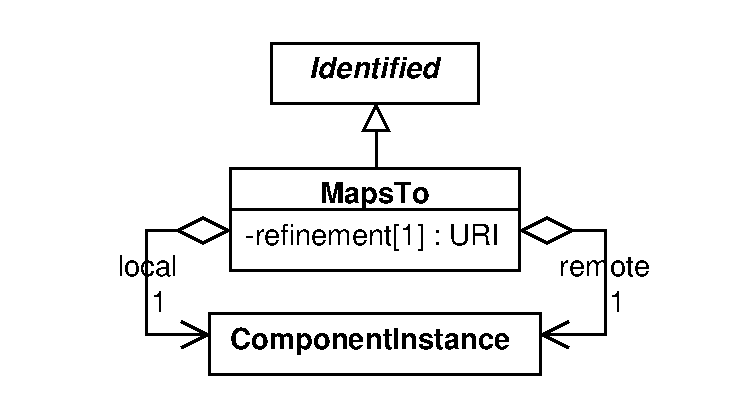
\includegraphics[scale=0.6]{uml/maps_to}
\caption[]{Diagram of the \sbol{MapsTo} class and its associated properties.}
\label{uml:maps_to}
\end{center}
\end{figure}

When \sbol{ComponentDefinition} and \sbol{ModuleDefinition} objects are composed into structural and functional hierarchies using \sbol{ComponentInstance} and \sbol{Module} objects, it is often the case that some \sbol{ComponentInstance} objects are intended to represent the same entity in the overall design. The purpose of the \sbol{MapsTo} class is to make these identity relationships clear and explicit.  For example, consider a \sbol{ModuleDefinition} for a genetic inverter that includes a \sbol{FunctionalComponent} for an abstract repressor protein.  When this \sbol{ModuleDefinition} is instantiated within a ``higher level'' \sbol{ModuleDefinition} that includes a \sbol{FunctionalComponent} for a LacI protein, the \sbol{MapsTo} object can be used to indicate that the repressor protein in the first \sbol{ModuleDefinition} is LacI in the context of the composite design.

In particular, a \sbol{MapsTo} object provides two pieces of information:
\begin{itemize}
\item An identity relationship between two \sbol{ComponentInstance} objects, the first contained by the ``lower level'' definition of the \sbol{ComponentInstance} or \sbol{Module} that owns the
  \sbol{MapsTo}, and the second contained by the ``higher level'' definition that contains the \sbol{ComponentInstance} or \sbol{Module} that owns the \sbol{MapsTo}. The \sbol{remote} property of a \sbol{MapsTo} refers to the first ``lower level'' \sbol{ComponentInstance}, while the \sbol{local} property refers to the second ``higher level'' \sbol{ComponentInstance}.
\item Instructions on how to interpret \sbol{local} and \sbol{remote} \sbol{ComponentInstance} objects that refer to different \sbol{ComponentDefinition} objects (that is, non-identical objects). These are specified using the \sbol{refinement} property of the \sbol{MapsTo} class.
\end{itemize}

\begin{figure}[ht]
\begin{center}
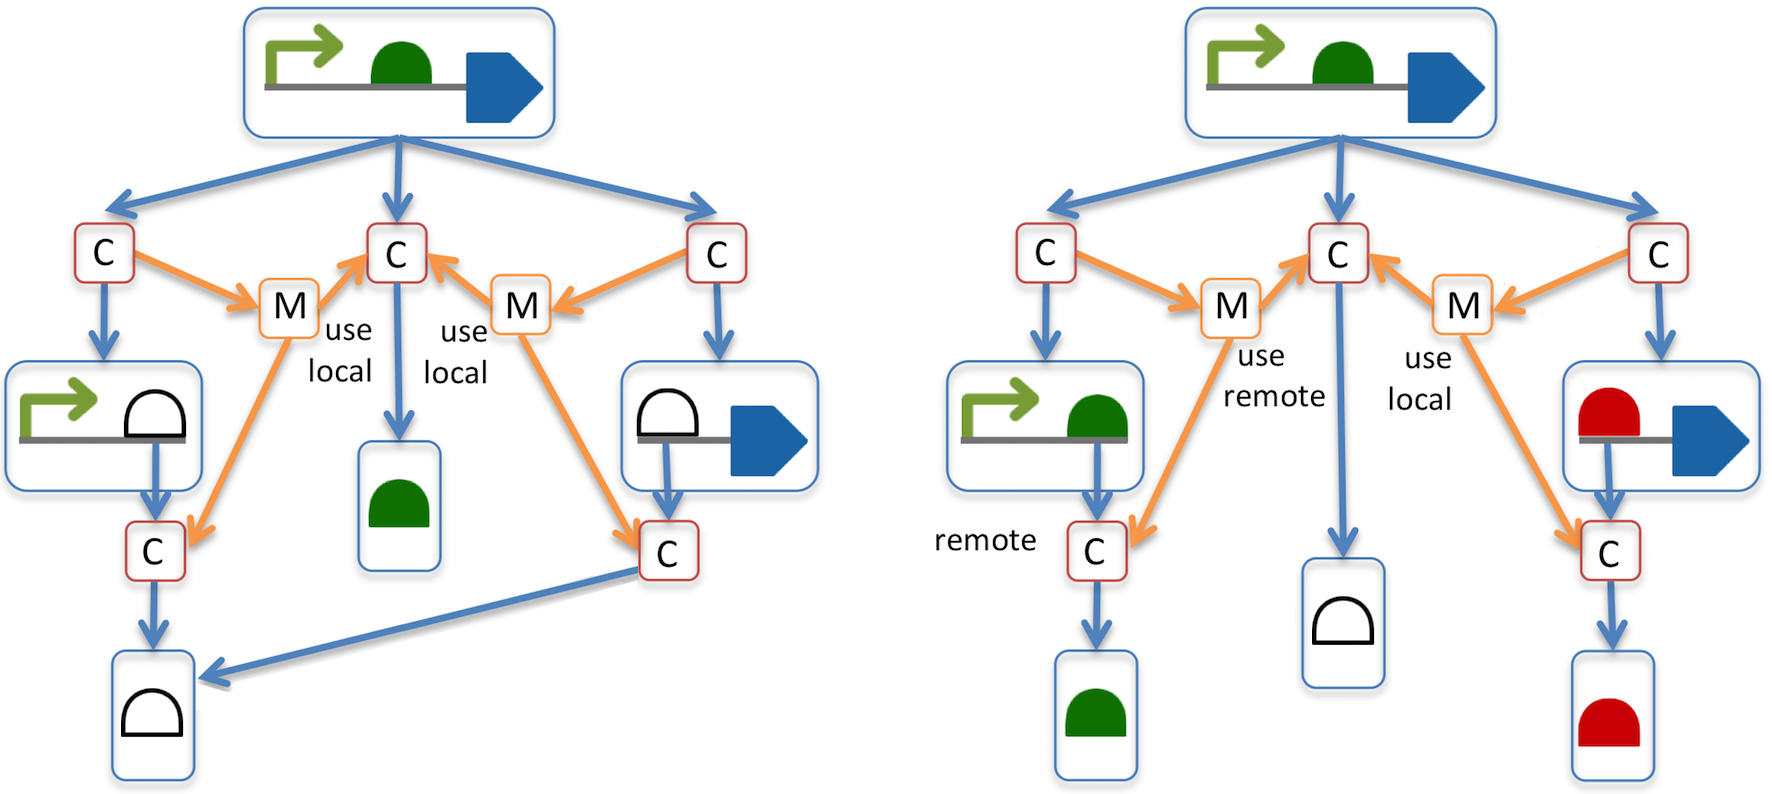
\includegraphics[scale=1]{images/MapsTo_Diagram3}
\caption{Linking \sbol{Component} objects using \sbol{MapsTo} entities. Boxes with diagrams represent \sbol{ComponentDefinition} objects, boxes with the C label represent \sbol{Component} objects, and boxes with the M label represent \sbol{MapsTo} objects. In both diagrams, a promoter-RBS \sbol{ComponentDefinition} and a RBS-CDS \sbol{ComponentDefinition} are being composed to form the \sbol{ComponentDefinition} of a complete transcriptional unit. In the left-hand diagram, the two \sbol{Component} objects inside the promoter-RBS \sbol{ComponentDefinition} and RBS-CDS \sbol{ComponentDefinition} objects both refer to an abstract RBS \sbol{ComponentDefinition} that lacks a sequence (white semicircle). Through the use of \sbol{MapsTo} objects with \sbol{refinement} set to useLocal, these ``lower level'' \sbol{ComponentDefinition} objects are effectively overridden by that of the green RBS in the \sbol{ComponentDefinition} of the complete transcriptional unit. In the right-hand diagram, however, the two ``lower level'' RBS \sbol{ComponentDefinition} objects do not lack sequences and it is the ``higher level'' RBS \sbol{ComponentDefinition} that is abstract. In this case, one of the \sbol{MapsTo} objects has a useRemote \sbol{refinement}, resulting in the green RBS \sbol{ComponentDefinition} overriding that of the abstract RBS in the ``higher level'' \sbol{ComponentDefinition}.}
\label{image:maps_to_diagram2}
\end{center}
\end{figure}

To illustrate this concept, two examples are provided in \ref{image:maps_to_diagram2}, in which the \sbol{ComponentDefinition} of a transcriptional unit is specified by composing two ``lower level'' \sbol{ComponentDefinition} objects.
In both examples, the two ``lower level'' \sbol{ComponentDefinition} objects each contain a RBS \sbol{Component} that is intended to represent the same design entity in the ``higher level'' \sbol{ComponentDefinition} of the transcriptional unit.

In order to explicitly represent the identity relationships in this example, a new RBS \sbol{Component} needs to be created inside the ``higher level'' \sbol{ComponentDefinition}.
This ``higher level'' \sbol{Component} then needs to be linked to the equivalent ``lower level'' \sbol{Component} objects by means of the \sbol{MapsTo} class, using one \sbol{MapsTo} object per link.
For example, in order to link the ``higher level'' RBS \sbol{Component} to the ``lower level'' RBS \sbol{Component} of the promoter-RBS \sbol{ComponentDefinition}, a \sbol{MapsTo} has to be created on the ``higher level'' promoter-RBS \sbol{Component}. The \sbol{local} property of this \sbol{MapsTo} then has to refer to the ``higher level'' RBS \sbol{Component}, while its \sbol{remote} property has to refer to the ``lower level'' RBS \sbol{Component}.
In this way, many ``lower level'' \sbol{Component} objects can be linked together at the ``higher level'' using as an equal number of \sbol{MapsTo} objects, each one referring to a different \sbol{remote} \sbol{Component}, but all referring to the same \sbol{local} \sbol{Component}.

The same types of identity relationships can also be declared between \sbol{FunctionalComponent} objects contained by \sbol{ModuleDefinition} objects, or between \sbol{Component} objects and \sbol{FunctionalComponent} objects contained by \sbol{ComponentDefinition} objects and \sbol{ModuleDefinition} objects, respectively. See \ref{sec:examples} and \ref{ser:examples} for additional examples using the \sbol{MapsTo} class.

\paragraph{The \sbolheading{local} property}\label{sec:local}
This REQUIRED property has a data type of \sbol{URI} and is used to refer to the \sbol{ComponentInstance} contained by the ``higher level'' \sbol{ComponentDefinition} or \sbol{ModuleDefinition}. This \sbol{local} \sbol{ComponentInstance} MUST be contained by the \sbol{ComponentDefinition} or \sbol{ModuleDefinition} that contains the \sbol{ComponentInstance} or \sbol{Module} that owns the \sbol{MapsTo}.

\paragraph{The \sbolheading{remote} property}\label{sec:remote}
This REQUIRED property has a data type of \sbol{URI} and is used to refer to the \sbol{ComponentInstance} contained by the ``lower level'' \sbol{ComponentDefinition} or \sbol{ModuleDefinition}.
This \sbol{remote} \sbol{ComponentInstance} MUST be contained by the \sbol{ComponentDefinition} or \sbol{ModuleDefinition} that is the \sbolmult{definition:CI}{definition} of the \sbol{ComponentInstance} or \sbol{Module} that owns the \sbol{MapsTo}.
Lastly, the \sbol{access} property of the \sbol{remote} \sbol{ComponentInstance} MUST be set to ``public.''

\paragraph{The \sbolheading{refinement} property}\label{sec:refinement}
The \sbol{refinement} property is REQUIRED and has a data type of \sbol{URI}. Each \sbol{MapsTo} object MUST specify the relationship between its \sbol{local} and \sbol{remote} \sbol{ComponentInstance} objects using one of the REQUIRED \sbol{refinement} \sbol{URI}s provided in \ref{tbl:mapsto_refinement}.
\twozeroone{Note that if multiple \sbol{MapsTo}s belonging to the \sbol{Component}s of a \sbol{ComponentDefinition} have \sbol{local} properties that refer to the same \sbol{Component}, then there MUST NOT be more than one such \sbol{MapsTo} that has a \sbol{refinement} property that contains the \sbol{URI} \url{http://sbols.org/v2\#useRemote}. Similarly, if multiple \sbol{MapsTo}s belonging the \sbol{Module}s and \sbol{FunctionalComponent}s of a \sbol{ModuleDefinition} have \sbol{local} properties that refer to the same \sbol{FunctionalComponent}, then there MUST NOT be more than one such \sbol{MapsTo} that has a \sbol{refinement} property that contains the \sbol{URI} \url{http://sbols.org/v2\#useRemote}.}


\begin{table}[ht]
  \begin{edtable}{tabular}{lp{4in}}
    \toprule
    \textbf{Refinement URI} & \textbf{Description} \\
    \midrule
    \url{http://sbols.org/v2#useRemote}  & All references to the \sbol{local}  \sbol{ComponentInstance} MUST dereference to the \sbol{remote} \sbol{ComponentInstance} instead.\\
    \url{http://sbols.org/v2#useLocal}  & In the context of the \sbol{ComponentDefinition} or \sbol{ModuleDefinition} that contains the owner of the \sbol{MapsTo}, all references to the \sbol{remote}  \sbol{ComponentInstance} MUST dereference to the \sbol{local} \sbol{ComponentInstance} instead.\\
    \url{http://sbols.org/v2#verifyIdentical}  & The \sbolmult{definition:CI}{definition} properties of the \sbol{local} and \sbol{remote} \sbol{ComponentInstance} objects MUST refer to the same \sbol{ComponentDefinition}.\\
        \url{http://sbols.org/v2#merge}  & In the context of the \sbol{ComponentDefinition} or \sbol{ModuleDefinition} that contains the owner of the \sbol{MapsTo}, all references to the \sbol{local} \sbol{ComponentInstance} or the \sbol{remote} \sbol{ComponentInstance} MUST dereference to both objects.\\
    \bottomrule
  \end{edtable}
  \caption{REQUIRED \sbol{URI}s for the \sbol{refinement} property.}
  \label{tbl:mapsto_refinement}
\end{table}

\paragraph{Serialization}
The serialization of \sbol{MapsTo} MUST have the following form.
\lstsetsbol
\begin{lstlisting}
<sbol:MapsTo rdf:about="...">
  ... [\emph{properties inherited from identified}] ...
  [\emph{one}] <sbol:refinement rdf:resource="..."/> [\emph{element}]
  [\emph{one}] <sbol:remote rdf:resource="..."/> [\emph{element}]
  [\emph{one}] <sbol:local rdf:resource="..."/> [\emph{element}]
</sbol:MapsTo>
\end{lstlisting}

In the example below, a \sbol{FunctionalComponent} in a ``higher level'' \sbol{ModuleDefinition} of a genetic toggle switch is linked to a \sbol{FunctionalComponent} in a ``lower level'' LacI inverter \sbol{ModuleDefinition}. The full example can be found in \ref{ser:toggleswitch}.
\lstsetsbol
\begin{lstlisting}
<sbol:MapsTo rdf:about="http://sbolstandard.org/example/toggle_switch/laci_inverter/LacI_mapping">
  <sbol:persistentIdentity rdf:resource="http://sbolstandard.org/example/toggle_switch/laci_inverter/LacI_mapping"/>
  <sbol:displayId>LacI_mapping</sbol:displayId>
  <sbol:refinement rdf:resource="http://sbols.org/v2#useRemote"/>
  <sbol:remote rdf:resource="http://sbolstandard.org/example/laci_inverter/TF"/>
  <sbol:local rdf:resource="http://sbolstandard.org/example/toggle_switch/LacI"/>
</sbol:MapsTo>
\end{lstlisting}


\subsubsection{SequenceAnnotation}
\label{sec:SequenceAnnotation}
The \sbol{SequenceAnnotation} class describes one or more regions of interest on the \sbol{Sequence} objects referred to by its parent \sbol{ComponentDefinition}. In addition, \sbol{SequenceAnnotation} objects can describe the substructure of their parent \sbol{ComponentDefinition} through association with the \sbol{Component} objects contained by this \sbol{ComponentDefinition}.

\begin{figure}[ht]
\begin{center}
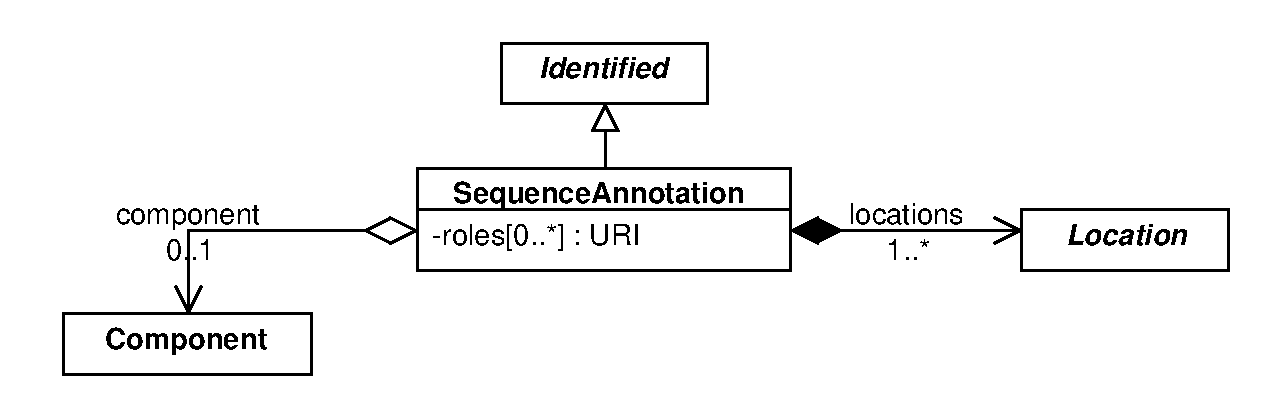
\includegraphics[scale=0.6]{uml/sequence_annotation}
\caption[]{Diagram of the \sbol{SequenceAnnotation} class and its associated properties.}
\label{uml:sequence_annotation}
\end{center}
\end{figure}

\paragraph{The \sbolheading{locations} property}\label{sec:locations}
The \sbol{locations} property is a REQUIRED set of one or more \sbol{Location} objects that indicate which \sbol{elements} of a \sbol{Sequence} are described by the \sbol{SequenceAnnotation}.

Allowing multiple \sbol{Location} objects on a single \sbol{SequenceAnnotation} is intended to enable representation of discontinuous regions (for example, a \sbol{Component} encoded across a set of exons with interspersed introns).
As such, the \sbol{Location} objects of a single \sbol{SequenceAnnotation} SHOULD NOT specify overlapping regions, since it is not clear what this would mean.
There is no such concern with different \sbol{SequenceAnnotation} objects, however, which can freely overlap in \sbol{Location} (for example, specifying overlapping linkers for sequence assembly).

\paragraph{The \sbolheading{component} property}\label{sec:component}
The \sbol{component} property is OPTIONAL and has a data type of \sbol{URI}. This \sbol{URI} MUST refer to a \sbol{Component} that is contained by the same parent \sbol{ComponentDefinition} that contains the \sbol{SequenceAnnotation}. In this way, the properties of the \sbol{SequenceAnnotation}, such as its \sbol{description} and \sbol{locations}, are associated with part of the substructure of its parent \sbol{ComponentDefinition}.

\twoonezero{
\paragraph{The \sbolheading{roles} property}\label{sec:roles:SA}
\vspace{-7pt}
\-\hspace{0.8cm}[New in 2.1.0; see SEP 004: \url{https://github.com/SynBioDex/SEPs/issues/4}]

The expected purpose and function of a genetic part are described by the
\sbolmult{roles:CD}{roles} property of \sbol{ComponentDefinition}. However, the
same building block might be used for a different purpose in an actual
design. In other words, purpose and function are sometimes determined by context. 

The \sbolmult{roles:SA}{roles} property comprises an OPTIONAL set of zero or more \sbol{URI}s describing the purpose or potential function of a given subsequence (and, if given, a sub-\sbol{ComponentDefinition} included by the associated \sbol{Component}) in the \textit{context} of its parent \sbol{ComponentDefinition}.
If provided, these \sbolmult{roles:SA}{role} \sbol{URI}s MUST identify terms from appropriate ontologies. Roles are not restricted to describing biological function; they may annotate \sbol{Sequence}s' function in any domain for which an ontology exists.

It is RECOMMENDED that these \sbolmult{roles:SA}{role} \sbol{URI}s identify terms that are compatible with the \sbolmult{types:CD}{type} properties of both this \sbol{SequenceAnnotation}'s' parent \sbol{ComponentDefinition} and, if given, the sub-\sbol{ComponentDefinition} included by the associated \sbol{Component}. For example, a \sbolmult{roles:SA}{role} of a \sbol{SequenceAnnotation} which belongs to a \sbol{ComponentDefinition} of type DNA and includes a sub-\sbol{ComponentDefinition} of type DNA might refer to terms from the Sequence Ontology. A table of recommended ontology terms for \sbolmult{roles:SA}{roles} is given in \ref{tbl:componentdefinition_roles}.
}

\twoonezero{
\paragraph{The \sbolheading{roleIntegration} property}\label{sec:roleIntegration:SA}
\vspace{-7pt}
\-\hspace{0.8cm}[New in 2.1.0; see SEP 004: \url{https://github.com/SynBioDex/SEPs/issues/4}]

A \sbolmult{roleIntegration:SA}{roleIntegration} specifies the relationship between a \sbol{SequenceAnnotation}'s own set of \sbolmult{roles:C}{roles} and the set of \sbolmult{roles:CD}{roles} on an associated \sbol{Component}.
The integrated result set of computed roles may even include \sbolmult{roles:CD}{role} elements from the associated \sbol{Component}'s sub-\sbol{ComponentDefinition} if dictated by the associated \sbol{Component}'s \sbolmult{roleIntegration:C}{roleIntegration} value. To determine the integrated role set for a \sbol{SequenceAnnotation}, first compute the integrated set of roles for this \sbol{SequenceAnnotation}'s associated \sbol{Component} according to the integration rules in the subsection on \sbolmult{roleIntegration:C}{Component.roleIntegration}. If there is no associated \sbol{Component}, then the associated set is assumed to be the empty set. After computing the associated set of \sbolmult{roles:CD}{roles}, compute the effective roles for this \sbol{SequenceAnnotation} by combining the associated set of \sbolmult{roles:CD}{roles} with this \sbol{SequenceAnnotation}'s own set of \sbolmult{roles:SA}{roles} according to the role integration rules.

The \sbolmult{roleIntegration:SA}{roleIntegration} property has a data type of \sbol{URI}. A \sbol{SequenceAnnotation} instance with zero \sbolmult{roles:SA}{roles} MAY OPTIONALLY specify a \sbolmult{roleIntegration:SA}{roleIntegration}. A \sbol{SequenceAnnotation} instance with one or more \sbolmult{roles:SA}{roles} MUST specify a \sbolmult{roleIntegration:SA}{roleIntegration} from \ref{tbl:sequenceAnnotation_roleIntegration}.
If zero \sbolmult{roles:SA}{roles} are given and no \sbolmult{roleIntegration:SA}{roleIntegration} is given, then \url{http://sbols.org/v2\#mergeRoles} is assumed.
It is RECOMMENDED to specify a set of \sbolmult{roles:SA}{roles} only if the integrated result set of roles would differ from the integrated set of roles computed for this \sbol{SequenceAnnotation}'s associated \sbol{Component}.
}

\twoonezero{
\begin{table}[ht]
  \begin{edtable}{tabular}{lp{4in}}
    \toprule
    \textbf{roleIntegration URI} & \textbf{Description} \\
    \midrule
    \url{http://sbols.org/v2\#overrideRoles} & In the context of this \sbol{SequenceAnnotation}, ignore the integrated set of roles computed for the associated \sbol{Component} (if given). Instead use only the set of zero or more \sbolmult{roles:SA}{roles} given for this \sbol{SequenceAnnotation}. \\
    \url{http://sbols.org/v2\#mergeRoles} & Use the union of the two sets: both the set of zero or more \sbolmult{roles:SA}{roles} given for this \sbol{SequenceAnnotation} as well as the integrated set of zero or more roles computed for the associated \sbol{Component} (if given). \\
    \bottomrule
  \end{edtable}
  \caption{\label{tbl:sequenceAnnotation_roleIntegration}
Each \sbolmult{roleIntegration:SA}{roleIntegration} mode is associated with a rule governing how a SequenceAnnotation's roles are to be combined with an associated Component's roles.}
\end{table}
}

\paragraph{Serialization}

\twoonezero{
The serialization of a \sbol{SequenceAnnotation} MUST have the form below. In this template, {\tt A\_LOCATION\_SUBCLASS} represents one of the \sbol{Location} subclasses.
}
\lstsetsbol
\begin{lstlisting}
<sbol:SequenceAnnotation rdf:about="...">
  ... [\emph{properties inherited from identified}] ...
  [\emph{zero or one}] <sbol:component rdf:resource="..."/> [\emph{element}]
  [\emph{one or more}] <sbol:location>
                 <sbol:A_LOCATION_SUBCLASS rdf:about="...">...</sbol:A_LOCATION_SUBCLASS>
              </sbol:location> [\emph{elements}]
  [\emph{zero or more}] <sbol:role rdf:resource="..."/> [\emph{elements}]
  [\emph{zero or one}]  <sbol:roleIntegration rdf:resource="..."/> [\emph{element}]
</sbol:SequenceAnnotation>
\end{lstlisting}

The example below shows the serialization of a \sbol{SequenceAnnotation} object. It specifies the region occupied by  a \sbol{Component} named BBa\_F2620.
\lstsetsbol
\begin{lstlisting}
<sbol:SequenceAnnotation rdf:about="http://partsregistry.org/cd/BBa_F2620/anno2">
  <sbol:persistentIdentity rdf:resource="http://partsregistry.org/cd/BBa_F2620/anno2"/>
  <sbol:displayId>anno2</sbol:displayId>
  <sbol:location>
    <sbol:Range rdf:about="http://partsregistry.org/cd/BBa_F2620/anno2/range">
      <sbol:persistentIdentity rdf:resource="http://partsregistry.org/cd/BBa_F2620/anno2/range"/>
      <sbol:displayId>range</sbol:displayId>
      <sbol:start>56</sbol:start>
      <sbol:end>68</sbol:end>
      <sbol:orientation rdf:resource="http://sbols.org/v2#inline"/>
    </sbol:Range>
  </sbol:location>
  <sbol:component rdf:resource="http://partsregistry.org/cd/BBa_F2620/rbs"/>
</sbol:SequenceAnnotation>
\end{lstlisting}

\subsubsection{Location}
\label{sec:Location}
The \sbol{Location} class is extended by the \sbol{Range}, \sbol{Cut}, and \sbol{GenericLocation} classes.

\begin{figure}[ht]
\begin{center}
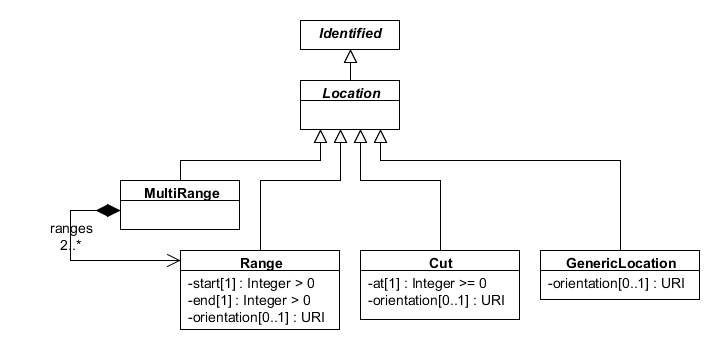
\includegraphics[scale=0.6]{uml/location}
\caption[]{Diagram of the \sbol{Location} class and its associated properties.}
\label{uml:location}
\end{center}
\end{figure}

\paragraph{The \sbolheading{orientation} property}
\label{sec:orientation}
The \sbol{orientation} property is OPTIONAL and has a data type of \sbol{URI}. All subclasses of \sbol{Location} share this property, which can be used to indicate how the region specified by the \sbol{SequenceAnnotation} and any associated double-stranded \sbol{Component} is oriented on the \sbol{elements} of a \sbol{Sequence}  from their parent \sbol{ComponentDefinition}. \ref{tbl:orientation_types} provides a list of REQUIRED \sbol{orientation} \sbol{URI}s. If a \sbol{Location} object has an \sbol{orientation}, then it MUST come from \ref{tbl:orientation_types}.

\begin{table}[ht]
  \begin{edtable}{tabular}{lp{3.75in}}
    \toprule
    \textbf{Orientation URI} & \textbf{Description} \\
    \midrule
    \url{http://sbols.org/v2\#inline} & The region specified by this \sbol{Location} is on the \sbol{elements} of a \sbol{Sequence}. \\
    \url{http://sbols.org/v2\#reverseComplement} & The region specified by this \sbol{Location} is on the reverse-complement translation of the \sbol{elements} of a \sbol{Sequence}. The exact nature of this translation depends on the \sbol{encoding} of the \sbol{Sequence}. \\
    \bottomrule
  \end{edtable}
  \caption{REQUIRED \sbol{URI}s for the \sbol{orientation} property}
  \label{tbl:orientation_types}
\end{table}


\paragraph{Range}
\label{sec:Range}
A \sbol{Range} object specifies a region via discrete, inclusive \sbol{start} and \sbol{end} positions that correspond to indices for characters in the \sbol{elements} \sbol{String} of a \sbol{Sequence}.

Note that the index of the first location is 1, as is typical practice in biology, rather than 0, as is typical practice in computer science.

\paragraph{The \sbolheading{start} property}\label{sec:start}
The \sbol{start} property specifies the inclusive starting position of the \sbol{Range}. This property is REQUIRED and MUST contain an \sbol{Integer} value greater than zero.

\paragraph{The \sbolheading{end} property}\label{sec:end}
The \sbol{end} property specifies the inclusive ending position of the \sbol{Range}. This property is REQUIRED and MUST contain an \sbol{Integer} value greater than zero. In addition, this \sbol{Integer} value MUST be greater than or equal to that of the \sbol{start} property.

\paragraph{Serialization}

The serialization of a \sbol{Range} MUST have the following form:
\lstsetsbol
\begin{lstlisting}
<sbol:Range rdf:about="...">
  ... [\emph{properties inherited from identified}] ...
  [\emph{one}]         <sbol:start>...</sbol:start> [\emph{element}]
  [\emph{one}]         <sbol:end>...</sbol:end> [\emph{element}]
  [\emph{zero or one}] <sbol:orientation rdf:resource="..."/> [\emph{element}]
</sbol:Range>
\end{lstlisting}

The example below shows the serialization of a \sbol{Range} object. It specifies the region between the inclusive positions 56 and 68, with an \sbol{orientation} of ``inline.''
\lstsetsbol
\begin{lstlisting}
<sbol:Range rdf:about="http://partsregistry.org/cd/BBa_F2620/anno2/range">
  <sbol:persistentIdentity rdf:resource="http://partsregistry.org/cd/BBa_F2620/anno2/range"/>
  <sbol:displayId>range</sbol:displayId>
  <sbol:start>56</sbol:start>
  <sbol:end>68</sbol:end>
  <sbol:orientation rdf:resource="http://sbols.org/v2#inline"/>
</sbol:Range>
\end{lstlisting}

\paragraph{Cut}
\label{sec:Cut}
The \sbol{Cut} class has been introduced to enable the specification of a region between two discrete positions.
This specification is accomplished using the \sbol{at} property, which specifies a discrete position that that corresponds to the index of a character in the \sbol{elements} \sbol{String} of a \sbol{Sequence} (except in the case when \sbol{at} is equal to zero---see below).

\paragraph{The \sbolheading{at} property}
\label{sec:at}
The \sbol{at} property is REQUIRED and MUST contain an \sbol{Integer} value greater than or equal to zero. The region specified by the \sbol{Cut} is between the position specified by this property and the position that immediately follows it. When the \sbol{at} property is equal to zero, the specified region is immediately before the first discrete position or character in the \sbol{elements} \sbol{String} of a \sbol{Sequence}.

\paragraph{Serialization}

The serialization of a \sbol{Cut} MUST have the following form:
\lstsetsbol
\begin{lstlisting}
<sbol:Cut rdf:about="...">
  ... [\emph{properties inherited from identified}] ...
  [\emph{one}]         <sbol:at>...</sbol:at> [\emph{element}]
  [\emph{zero or one}] <sbol:orientation rdf:resource="..."/> [\emph{element}]
</sbol:Cut>
\end{lstlisting}

The example below shows the serialization of a \sbol{Cut} object. It specifies a region in between positions 10 and 11, with an \sbol{orientation} of ``inline.''
\lstsetsbol
\begin{lstlisting}
<sbol:Cut rdf:about="http://partsregistry.org/cd/BBa_J23119/cutat10/cut">
  <sbol:persistentIdentity rdf:resource="http://partsregistry.org/cd/BBa_J23119/cutat10/cut"/>
  <sbol:displayId>cut</sbol:displayId>
  <sbol:at>10</sbol:at>
  <sbol:orientation rdf:resource="http://sbols.org/v2#inline"/>
</sbol:Cut>
\end{lstlisting}


\paragraph{GenericLocation}
\label{sec:GenericLocation}

While the \sbol{Range} and \sbol{Cut} classes are best suited to
specifying regions on \sbol{Sequence} objects with \external{IUPAC} encodings, the
\sbol{GenericLocation} class is included as a starting point for specifying regions on \sbol{Sequence} objects with different \sbol{encoding} properties and potentially nonlinear structure. This class can also be used to set the \sbol{orientation} of a \sbol{SequenceAnnotation} and any associated \sbol{Component} when their parent \sbol{ComponentDefinition} is a partial design that lacks a \sbol{Sequence}.

\paragraph{Serialization}

The serialization of a \sbol{GenericLocation} MUST have the following form:
\lstsetsbol
\begin{lstlisting}
<sbol:GenericLocation rdf:about="...">
  ... [\emph{properties inherited from identified}] ...
  [\emph{zero or one}] <sbol:orientation rdf:resource="..."/> [\emph{element}]
</sbol:GenericLocation>
\end{lstlisting}

The example below shows the serialization of a \sbol{GenericLocation} object with an \sbol{orientation} of ``reverse complement'':
\lstsetsbol
\begin{lstlisting}
<sbol:GenericLocation rdf:about="http://www.partsregistry.org/Part:BBa_F2620/anno5/location">
  <sbol:orientation rdf:resource="http://sbols.org/v2#reverseComplement"/>
</sbol:GenericLocation>
\end{lstlisting}

\subsubsection{SequenceConstraint}
\label{sec:SequenceConstraint}
The \sbol{SequenceConstraint} class can be used to assert restrictions on the relative, sequence-based positions of pairs of \sbol{Component} objects contained by the same parent \sbol{ComponentDefinition}.
The primary purpose of this class is to enable the specification of partially designed \sbol{ComponentDefinition} objects, for which the precise positions or orientations of their contained \sbol{Component} objects are not yet fully determined. Each \sbol{SequenceConstraint} includes the \sbol{restriction}, \sbol{subject}, and \sbol{object} properties.

\begin{figure}[ht]
\begin{center}
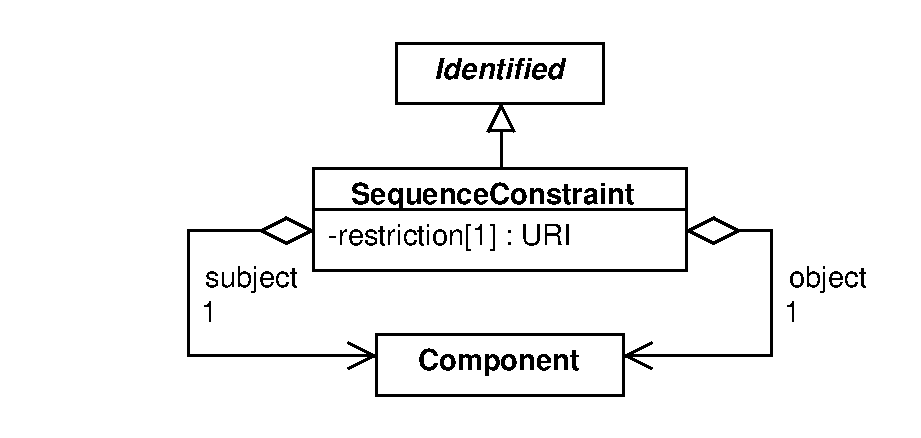
\includegraphics[scale=0.6]{uml/sequence_constraint}
\caption[]{Diagram of the \sbol{SequenceConstraint} class and its associated properties.}
\label{uml:sequence_constraint}
\end{center}
\end{figure}

\paragraph{The \sbolheading{subject} property}\label{sec:subject}
The \sbol{subject} property is REQUIRED and MUST contain a \sbol{URI} that refers to a \sbol{Component} contained by the same parent \sbol{ComponentDefinition} that contains the \sbol{SequenceConstraint}.

\paragraph{The \sbolheading{object} property}\label{sec:object}
The \sbol{object} property is REQUIRED and MUST contain a \sbol{URI} that refers to a \sbol{Component} contained by the same parent \sbol{ComponentDefinition} that contains the \sbol{SequenceConstraint}. This \sbol{Component} MUST NOT be the same \sbol{Component} that the \sbol{SequenceConstraint} refers to via its \sbol{subject} property.

\paragraph{The \sbolheading{restriction} property}\label{sec:restriction}

The \sbol{restriction} property is REQUIRED and has a data type of \sbol{URI}. This property MUST indicate the type of structural restriction on the relative, sequence-based positions or orientations of the \sbol{subject} and \sbol{object} \sbol{Component} objects. The \sbol{URI} value of this property SHOULD come from the RECOMMENDED \sbol{URI}s in  \ref{tbl:restriction_types}.

% Note: With regards to SBOL Version 1.1., this is a generalization of former \sbol{SequenceAnnotation} property \external{precedes}.

\begin{table}[ht]
  \begin{edtable}{tabular}{lp{4in}}
    \toprule
    \textbf{Restriction URI} & \textbf{Description} \\
    \midrule
    \url{http://sbols.org/v2\#precedes} & The position of the \sbol{subject} \sbol{Component} MUST precede that of the \sbol{object} \sbol{Component}. If each one is associated with a \sbol{SequenceAnnotation}, then the \sbol{SequenceAnnotation} associated with the \sbol{subject} \sbol{Component} MUST specify a region that starts before the region specified by the \sbol{SequenceAnnotation} associated with the \sbol{object} \sbol{Component}. \\
    \url{http://sbols.org/v2\#sameOrientationAs} & The \sbol{subject} and \sbol{object} \sbol{Component} objects MUST have the same orientation. If each one is associated with a \sbol{SequenceAnnotation}, then the \sbol{orientation} \sbol{URI}s of the \sbol{Location} objects of the first \sbol{SequenceAnnotation} MUST be among those of the second \sbol{SequenceAnnotation}, and vice versa. \\
    \url{http://sbols.org/v2\#oppositeOrientationAs} & The \sbol{subject} and \sbol{object} \sbol{Component} objects MUST have opposite orientations. If each one is associated with a \sbol{SequenceAnnotation}, then the \sbol{orientation} \sbol{URI}s of the \sbol{Location} objects of one \sbol{SequenceAnnotation} MUST NOT be among those of the other \sbol{SequenceAnnotation}. \\
    \bottomrule
  \end{edtable}
  \caption{RECOMMENDED \sbol{URI}s for the \sbol{restriction} property.}
  \label{tbl:restriction_types}
\end{table}

\paragraph{Serialization}

The serialization of a \sbol{SequenceConstraint} MUST have the following form:
\lstsetsbol
\begin{lstlisting}
<sbol:SequenceConstraint rdf:about="...">
  ... [\emph{properties inherited from identified}] ...
  [\emph{one}] <sbol:restriction rdf:resource="..."/> [\emph{element}]
  [\emph{one}] <sbol:subject rdf:resource="..."/> [\emph{element}]
  [\emph{one}] <sbol:object rdf:resource="..."/> [\emph{element}]
</sbol:SequenceConstraint>
\end{lstlisting}

The example below shows the serialization of a \sbol{SequenceConstraint} belonging to the \sbol{ComponentDefinition} of a LacI-repressible promoter. This \sbol{SequenceConstraint} has a ``precedes'' \sbol{restriction} that indicates that the \sbol{subject} \sbol{Component}, which represents the core of the promoter, is positioned before the \sbol{object} \sbol{Component}, which represents the LacI operator of the promoter.
\lstsetsbol
\begin{lstlisting}
<sbol:SequenceConstraint rdf:about="http://partsregistry.org/cd/BBa_K174004/r1">
  <sbol:persistentIdentity rdf:resource="http://partsregistry.org/cd/BBa_K174004/r1"/>
  <sbol:displayId>r1</sbol:displayId>
  <sbol:restriction rdf:resource="http://sbols.org/v2#precedes"/>
  <sbol:subject rdf:resource="http://partsregistry.org/cd/pspac"/>
  <sbol:object rdf:resource="http://partsregistry.org/cd/LacI_operator"/>
</sbol:SequenceConstraint>
\end{lstlisting}

\subsection{Model}
\label{sec:Model}

\begin{figure}[ht]
\begin{center}
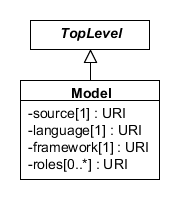
\includegraphics[scale=0.6]{uml/model}
\caption[]{Diagram of the \sbol{Model} class and its associated properties.}
\label{uml:model}
\end{center}
\end{figure}

The purpose of the \sbol{Model} class is to serve as a placeholder for an external computational model and provide additional meta-data to enable better reasoning about the contents of this model.
In this way, there is minimal duplication of standardization efforts and users of SBOL can formalize the function of a \sbol{ModuleDefinition} in the language of their choice.

The meta-data provided by the \sbol{Model} class include the following properties: the \sbol{source} or location of the actual content of the model, the \sbol{language} in which the model is implemented, and the model's \sbol{framework}.

\subsubsection*{ The \sbolheading{source} property}\label{sec:source}
The \sbol{source} property is REQUIRED and MUST contain a \sbol{URI} reference to the source file for a model.

\subsubsection*{ The \sbolheading{language} property}\label{sec:language}
The \sbol{language} property is REQUIRED and MUST contain a \sbol{URI} that specifies the language in which the model is implemented. It is RECOMMENDED that this \sbol{URI} refer to a term from the EMBRACE Data and Methods (EDAM) ontology. \ref{tbl:model_types} provides a list of terms from this ontology and their \sbol{URI}s. If the \sbol{language} property of a \sbol{Model} is well-described by one these terms, then it MUST contain the \sbol{URI} for this term as its value.

\begin{table}[ht]
  \begin{edtable}{tabular}{ll}
    \toprule
    \textbf{Model Language} & \textbf{URI for EDAM Term} \\
    \midrule
    SBML  & \url{http://identifiers.org/edam/format_2585}\\
    CellML		 & \url{http://identifiers.org/edam/format_3240}\\
    BioPAX    & \url{http://identifiers.org/edam/format_3156}\\
    \bottomrule
  \end{edtable}
  \caption{Terms from the EDAM ontology to specify the \sbol{language} property of a \sbol{Model}.}
  \label{tbl:model_types}
\end{table}


\subsubsection*{ The \sbolheading{framework} property}\label{sec:framework}
The \sbol{framework} property is REQUIRED and MUST contain a \sbol{URI} that specifies the framework in which the model is implemented.
It is RECOMMENDED this \sbol{URI} refer to a term from the modeling framework branch of the SBO when possible. A few suggested modeling frameworks and their corresponding \sbol{URI}s are shown in \ref{tbl:model_frameworks}. If the \sbol{framework} property of a \sbol{Model} is well-described by one these terms, then it MUST contain the \sbol{URI} for this term as its value.

\begin{table}[ht]
  \begin{edtable}{tabular}{ll}
    \toprule
    \textbf{Framework} & \textbf{URI for SBO Term} \\
    \midrule
    Continuous  & \url{http://identifiers.org/biomodels.sbo/SBO:0000062}\\
    Discrete & \url{http://identifiers.org/biomodels.sbo/SBO:0000063}\\
    \bottomrule
  \end{edtable}
  \caption{SBO terms to specify the \sbol{framework} property of a \sbol{Model}.}
  \label{tbl:model_frameworks}
\end{table}

\subsubsection*{Serialization}

The serialization of a \sbol{Model} MUST have the following form:

\lstsetsbol
\begin{lstlisting}
<sbol:Model rdf:about="http://www.sbolstandard.org/examples/toggleswitch">
  ... [\emph{properties inherited from identified}] ...
  [\emph{one}] <sbol:source rdf:resource="..."/> [\emph{element}]
  [\emph{one}] <sbol:language rdf:resource="..."/> [\emph{element}]
  [\emph{one}] <sbol:framework rdf:resource="..."/> [\emph{element}]
</sbol:Model>
\end{lstlisting}

The example below shows the serialization of a \sbol{Model} object that refers to a quantitative model of a genetic toggle switch. The model is implemented in the SBML \sbol{language} and adheres to a continuous modeling \sbol{framework}. Lastly, the model can be retrieved from a model repository via its \sbol{source} \sbol{URI}, which is a \external{URL}.
\lstsetsbol
\begin{lstlisting}
<?xml version="1.0" ?>
<rdf:RDF xmlns:rdf="http://www.w3.org/1999/02/22-rdf-syntax-ns#" xmlns:dcterms="http://purl.org/dc/terms/" xmlns:prov="http://www.w3.org/ns/prov#" xmlns:sbol="http://sbols.org/v2#">
  <sbol:Model rdf:about="http://www.sbolstandard.org/examples/pIKE_Toggle_1">
    <sbol:persistentIdentity rdf:resource="http://www.sbolstandard.org/examples/pIKE_Toggle_1"/>
    <sbol:displayId>pIKE_Toggle_1</sbol:displayId>
    <dcterms:title>pIKE_Toggle_1 toggle switch</dcterms:title>
    <sbol:source rdf:resource="http://virtualparts.org/part/pIKE_Toggle_1"/>
    <sbol:language rdf:resource="http://identifiers.org/edam/format_2585"/>
    <sbol:framework rdf:resource="http://identifiers.org/biomodels.sbo/SBO:0000062"/>
  </sbol:Model>
</rdf:RDF>
\end{lstlisting}
\label{ser:Model}

\subsection{ModuleDefinition}
\label{sec:ModuleDefinition}

\begin{figure}[ht]
\begin{center}
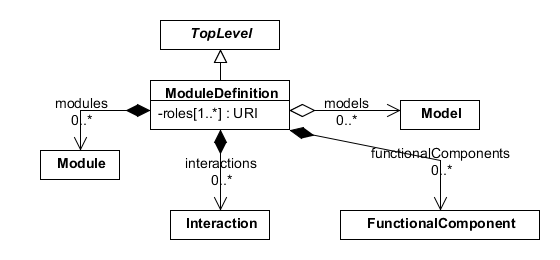
\includegraphics[scale=0.6]{uml/module_definition}
\caption[]{Diagram of the \sbol{ModuleDefinition} class and its associated properties.}
\label{uml:module_definition}
\end{center}
\end{figure}

The \sbol{ModuleDefinition} class represents a grouping of structural and functional entities in a biological design. The primary usage of this class is to assert the molecular interactions and abstract function of its child entities.

As shown in \ref{uml:module_definition}, these child entities are aggregated via the \sbol{functionalComponents} \sbol{modules} properties, while representation of their abstract function is accomplished via the \sbolmult{roles:MD}{roles}  property. More detailed descriptions of the function of a \sbol{ModuleDefinition} are provided by its \sbol{interactions} and \sbol{models} properties. Lastly, since \sbol{ModuleDefinition} objects can be more abstract and represent entities of  engineering design rather than biology, they can have designated ``inputs'' and ``outputs'' expressed by the \sbol{direction} properties on its \sbol{FunctionalComponent} objects.

\subsubsection*{The \sbolheading{roles} property}\label{sec:roles:MD}
The \sbolmult{roles:MD}{roles} property is an OPTIONAL set of \sbol{URI}s that clarifies the intended function of a \sbol{ModuleDefinition}.

These \sbol{URI}s might identify descriptive biological roles, such as ``metabolic pathway'' and ``signaling cascade,'' but they can also identify identify ``logical'' roles, such as ``inverter'' or ``AND gate'', or other abstract roles for describing the function of design. Interpretation of the meaning of such roles currently depends on the software tools that read and write them.

\subsubsection*{The \sbolheading{modules} property}\label{sec:modules}

The \sbol{modules} property is OPTIONAL and MAY specify a set of \sbol{Module} objects contained by the \sbol{ModuleDefinition}.
Note that the set of relations between \sbol{Module} and \sbol{ModuleDefinition} objects is strictly acyclic.

While the \sbol{ModuleDefinition} class is analogous to a specification sheet for a system of interacting biological elements, the \sbol{Module} class represents the occurrence of a particular subsystem within the system.
Hence, this class allows a system design to include multiple instances of a subsystem, all defined by reference to the same \sbol{ModuleDefinition}.
For example, consider the \sbol{ModuleDefinition} for a network of two-input repressor devices in which the particular repressors have not been chosen yet. This \sbol{ModuleDefinition} could contain multiple \sbol{Module} objects that refer to the same \sbol{ModuleDefinition} of an abstract two-input repressor device.

\subsubsection*{The \sbolheading{functionalComponents} property}
\label{sec:functionalComponents}

The \sbol{functionalComponents} property is OPTIONAL and MAY specify a set of \sbol{FunctionalComponent} objects contained by the \sbol{ModuleDefinition}.

Just as a \sbol{Module} represents an instance of a subsystem in the overall system represented by a  \sbol{ModuleDefinition}, a \sbol{FunctionalComponent} represents an instance of a structural entity (represented by a \sbol{ComponentDefinition}) in the system. This concept allows a \sbol{ModuleDefinition} to assert different interactions for separate copies of the same structural entity if needed. For example, a \sbol{ModuleDefinition} might contain multiple \sbol{FunctionalComponent}  objects that refer to the same promoter \sbol{ComponentDefinition}, but assert different interactions for these promoter copies based on their separate positions in another \sbol{ComponentDefinition} that represents the structure of the entire system.

\subsubsection*{The \sbolheading{interactions} property}\label{sec:interactions}

The \sbol{interactions} property is OPTIONAL and MAY specify a set of \sbol{Interaction} objects within the \sbol{ModuleDefinition}.

The \sbol{Interaction} class provides an abstract, machine-readable representation of entity behavior within a \sbol{ModuleDefinition} (whereas a more detailed model of the system might not be suited to machine reasoning, depending on its implementation).
Each \sbol{Interaction} contains \sbol{Participation} objects that indicate the roles of the \sbol{FunctionalComponent} objects involved in the \sbol{Interaction}.

\subsubsection*{The \sbolheading{models} property}\label{sec:models}
The \sbol{models} property is OPTIONAL and MAY specify a set of \sbol{URI} references to \sbol{Model} objects.

\sbol{Model} objects are placeholders that link \sbol{ModuleDefinition} objects to computational models of any format.
A \sbol{ModuleDefinition} object can link to more than one \sbol{Model} since each might encode system behavior in a different way or at a different level of detail.

\subsubsection*{Serialization}

The serialization of \sbol{ModuleDefinition} has the following form:
\lstsetsbol
\begin{lstlisting}
<sbol:ModuleDefinition rdf:about="...">
  ... [\emph{properties inherited from identified}] ...
  [\emph{zero or more}]  <sbol:role rdf:resource="..."/> [\emph{elements}]
  [\emph{zero or more}]  <sbol:model rdf:resource="..."/> [\emph{elements}]
  [\emph{zero or more}] <sbol:functionalComponent>
                 <sbol:FunctionalComponent rdf:about="...">...</sbol:FunctionalComponent >
               </sbol:functionalComponent> [\emph{elements}]
  [\emph{zero or more}] <sbol:module>
                 <sbol:Module rdf:about="...">...</sbol:Module>
               </sbol:module> [\emph{elements}]
  [\emph{zero or more}] <sbol:interaction>
                 <sbol:Interaction rdf:about="...">...</sbol:Interaction>
               </sbol:interaction> [\emph{elements}]
</sbol:ModuleDefinition>
\end{lstlisting}

The example below shows a simple \sbol{ModuleDefinition} containing two components, a \sbol{FunctionalComponent} for a DNA sequence encoding constitutive expression of GFP and another for the GFP protein expressed from this sequence, plus an interaction describing that relation.

\lstsetsbol
\begin{lstlisting}
<sbol:ModuleDefinition rdf:about="http://sbolstandard.org/example/md/GFP_expression">
  <sbol:functionalComponent>
    <sbol:FunctionalComponent rdf:about="http://sbolstandard.org/example/md/GFP_expression/GFP_protein">
      <sbol:definition rdf:resource="http://sbolstandard.org/example/GFP"/>
      <sbol:access rdf:resource="http://sbols.org/v2#public"/>
      <sbol:direction rdf:resource="http://sbols.org/v2#output"/>
    </sbol:FunctionalComponent>
  </sbol:functionalComponent>
  <sbol:functionalComponent>
    <sbol:FunctionalComponent rdf:about="http://sbolstandard.org/example/md/GFP_expression/Constitutive_GFP">
      <sbol:definition rdf:resource="http://sbolstandard.org/example/GFP_generator"/>
      <sbol:access rdf:resource="http://sbols.org/v2#public"/>
      <sbol:direction rdf:resource="http://sbols.org/v2#none"/>
    </sbol:FunctionalComponent>
  </sbol:functionalComponent>
  <sbol:interaction>
    <sbol:Interaction rdf:about="http://sbolstandard.org/example/md/GFP_expression/express_GFP">
      ...
    </sbol:Interaction>
  </sbol:interaction>
</sbol:ModuleDefinition>
\end{lstlisting}

\subsubsection{Module}
\label{sec:Module}

\begin{figure}[ht]
\begin{center}
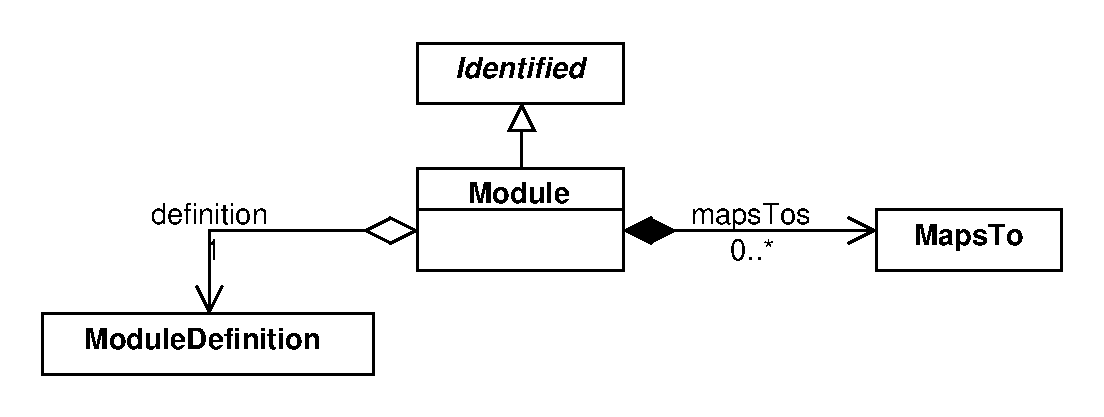
\includegraphics[scale=0.6]{uml/module}
\caption[]{Diagram of the \sbol{Module} class and its associated properties.}
\label{uml:module}
\end{center}
\end{figure}

The \sbol{Module} class represents the usage or occurrence of a \sbol{ModuleDefinition} within a larger design (that is, another \sbol{ModuleDefinition}).

\paragraph{The \sbolheading{definition} property}
\label{sec:definition:M}

The \sbolmult{definition:M}{definition} property is a REQUIRED \sbol{URI} that refers to the \sbol{ModuleDefinition} for the \sbol{Module}.

The \sbolmult{definition:M}{definition} property MUST NOT refer to the same \sbol{ModuleDefinition} as that which contains the \sbol{Module}.
Furthermore, \sbol{Module} objects MUST NOT form a cyclical chain of references via their \sbolmult{definition:M}{definition} properties and the \sbol{ModuleDefinition} objects that contain them. For example, consider the \sbol{Module} objects $A$ and $B$ and the \sbol{ModuleDefinition} objects $X$ and $Y$. The reference chain ``$X$ contains $A$, $A$ is defined by $Y$, $Y$ contains $B$, and $B$ is defined by $X$'' is cyclical.

\paragraph{The \sbolheading{mapsTo} property}
\label{sec:mapsTos:M}

The \sbolmult{mapsTos:M}{mapsTos} property is an OPTIONAL set of \sbol{MapsTo} objects that refer to and link \sbol{ComponentInstance} objects together within the heterarchy of \sbol{Module}, \sbol{ModuleDefinition}, \sbol{ComponentInstance}, and \sbol{ComponentDefinition} objects.

\ref{sec:MapsTo} contains a detailed description of the \sbol{MapsTo} class.

\paragraph{Serialization}
The serialization of \sbol{Module}s has the following form.
\lstsetsbol
\begin{lstlisting}
<sbol:Module rdf:about="...">
  ... [\emph{properties inherited from identified}] ...
  [\emph{one}]          <sbol:definition rdf:resource="..."/> [\emph{element}]
  [\emph{zero or more}] <sbol:mapsTo>
                 <sbol:MapsTo rdf:about="...">...</sbol:MapsTo>
               </sbol:mapsTo> [\emph{element}]
</sbol:Module>
\end{lstlisting}

The example below specifies a TetR inverter that is being used as
a part of a genetic toggle switch:

\lstsetsbol
\begin{lstlisting}
<sbol:Module rdf:about="http://sbolstandard.org/example/toggle_switch/tetr_inverter">
  <sbol:definition rdf:resource="http://sbolstandard.org/example/tetr_inverter"/>
  ...
</sbol:Module>
\end{lstlisting}

\subsubsection{FunctionalComponent}
\label{sec:FunctionalComponent}
A \sbol{FunctionalComponent} is an instance of a \sbol{ComponentDefinition} being used as part of a \sbol{ModuleDefinition}. The \sbol{ModuleDefinition} describes how the that describes how the \sbol{FunctionalComponent} interacts with others and summarizes their aggregate function.

The \sbol{FunctionalComponent} class inherits from the \sbol{ComponentInstance} class and therefore has the \sbolmult{definition:CI}{definition}, \sbol{access}, and \sbolmult{mapsTos:CI}{mapsTos} properties.
In addition, it has a \sbol{direction} property that specifies whether it serves as an input, output, both, or neither with regards to the \sbol{ModuleDefinition} that contains it.

\paragraph{The \sbolheading{direction} property}\label{sec:direction}
Each \sbol{FunctionalComponent} MUST specify via the \sbol{direction} property whether it serves as an  input, output, both, or neither for its parent \sbol{ModuleDefinition} object.
The value for this property MUST be one of the \sbol{URI}s given in \ref{tbl:functionalcomponent_directions}.


\begin{table}[ht]
  \begin{edtable}{tabular}{ll}
    \toprule
    \textbf{Direction URI} & \textbf{Description} \\
    \midrule

    \url{http://sbols.org/v2#in}  & Indicates that the \sbol{FunctionalComponent} is an input.\\
    \url{http://sbols.org/v2#out}  & Indicates that the \sbol{FunctionalComponent} is an output.\\
   \url{http://sbols.org/v2#inout}  & Indicates that the \sbol{FunctionalComponent} is both an input and output\\ \url{http://sbols.org/v2#none}  & Indicates that the \sbol{FunctionalComponent} is neither an input or output.\\
    \bottomrule
  \end{edtable}
  \caption{REQUIRED \sbol{URI}s for the \sbol{direction} property.}
  \label{tbl:functionalcomponent_directions}
\end{table}

The \sbol{direction} property is a means to encode how a  designer thinks about the ``purpose'' of a connection in a system.  In SBOL, such a connection is represented with a \sbol{FunctionalComponent}, and a system is represented as  with a \sbol{ModuleDefinition}.
For example, consider a system that has been designed to sense the concentration of the cell-to-cell signaling molecule 3OC$_6$HSL and report it via the concentration of another gene product.
In this system, the concentration of 3OC$_6$HSL is being sensed by the system, so the \sbol{FunctionalComponent} for 3OC$_6$HSL would have a \sbol{direction} of ``input.''
In turn, the concentration of the reporter gene product is intended to be read/consumed by other biological systems, so the \sbol{FunctionalComponent} for this product would have a \sbol{direction} of ``output.''
The CDS encoding the product, however, is not intended to directly transfer information into or out of the \sbol{ModuleDefinition} for the system, so its \sbol{FunctionalComponent} would have a \sbol{direction} of ``neither.''

\paragraph{Serialization}

The serialization of a \sbol{FunctionalComponent} has the following form.
\lstsetsbol
\begin{lstlisting}
<sbol:FunctionalComponent rdf:about="...">
  ... [\emph{properties inherited from identified}] ...
  [\emph{one}]          <sbol:definition rdf:resource="..."/> [\emph{element}]
  [\emph{one}]          <sbol:access rdf:resource="..."/> [\emph{element}]
  [\emph{one}]          <sbol:direction rdf:resource="..."/> [\emph{element}]
  [\emph{zero or more}] <sbol:mapsTo rdf:resource="..."/> [\emph{elements}]
</sbol:FunctionalComponent>
\end{lstlisting}

In the example below, the functional component is defined as a public input/output. The component refers to the \texttt{Part:BBa\_R0010} promoter from the iGEM Parts Registry.
\lstsetsbol
\begin{lstlisting}
<sbol:FunctionalComponent rdf:about="http://sbolstandard.org/example/laci_inverter/promoter">
  <sbol:definition rdf:resource="http://www.partsregistry.org/BBa_R0010"/>
  <sbol:access rdf:resource="http://sbols.org/v2#public"/>
  <sbol:direction rdf:resource="http://sbols.org/v2#inout"/>
</sbol:FunctionalComponent>
\end{lstlisting}

\subsubsection{Interaction}
\label{sec:Interaction}

\begin{figure}[ht]
\begin{center}
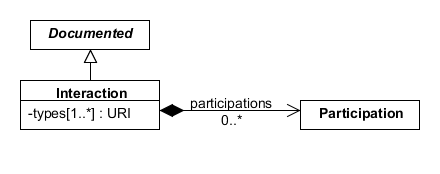
\includegraphics[scale=0.6]{uml/interaction}
\caption[]{Diagram of the \sbol{Interaction} class and its associated properties.}
\label{uml:interaction}
\end{center}
\end{figure}

The \sbol{Interaction} class provides more detailed description of how the \sbol{FunctionalComponent} objects of a \sbol{ModuleDefinition} are intended to work together.
For example, this class can be used to represent different forms of genetic regulation (e.g., transcriptional activation or repression), processes from the central dogma of biology (e.g. transcription and translation), and other basic molecular interactions (e.g., non-covalent binding or enzymatic phosphorylation).
Each \sbol{Interaction} includes a \sbolmult{types:I}{types} property that refers to descriptive ontology terms and a \sbol{participations} property that describes which \sbol{FunctionalComponent} objects participate in the \sbol{Interaction}.

\paragraph{The \sbolheading{types} property}\label{sec:types:I}

The \sbolmult{types:I}{types} property is a REQUIRED set of \sbol{URI}s that describes the behavior represented by an \sbol{Interaction}.

The \sbolmult{types:I}{types} property MUST contain one or more \sbol{URI}s that MUST identify terms from appropriate ontologies. It is RECOMMENDED that \twozeroone{exactly one \sbol{URI}} contained by the \sbolmult{types:I}{types} property refer to a term from the occurring entity branch of the Systems Biology Ontology (SBO). (See \url{http://www.ebi.ac.uk/sbo/main/}) \ref{tbl:interaction_types} provides a list of possible SBO terms for the \sbolmult{types:I}{types} property and their corresponding \sbol{URI}s.

\twozeroone{
\begin{table}[ht]
  \begin{edtable}{tabular}{ll}
    \toprule
    \textbf{Interaction Type} & \textbf{URI for SBO Term} \\
    \midrule
    Inhibition  & \url{http://identifiers.org/biomodels.sbo/SBO:0000169}\\
    Stimulation & \url{http://identifiers.org/biomodels.sbo/SBO:0000170}\\
    Biochemical Reaction & \url{http://identifiers.org/biomodels.sbo/SBO:0000176}\\
    Non-Covalent Binding & \url{http://identifiers.org/biomodels.sbo/SBO:0000177}\\
    Degradation & \url{http://identifiers.org/biomodels.sbo/SBO:0000179}\\
    Genetic Production & \url{http://identifiers.org/biomodels.sbo/SBO:0000589}\\
    \bottomrule
  \end{edtable}
  \caption{SBO terms to specify the \sbolmult{types:I}{types} property of an \sbol{Interaction}.}
  \label{tbl:interaction_types}
\end{table}
}

If an \sbol{Interaction} is well described by one of the terms from \ref{tbl:interaction_types}, then its \sbolmult{types:I}{types} property MUST contain the \sbol{URI} that identifies this term. Lastly, if the \sbolmult{types:I}{types} property of an \sbol{Interaction} contains multiple
 \sbol{URI}s, then they MUST identify non-conflicting terms. For example, the SBO terms ``stimulation'' and ``inhibition'' would conflict.

\paragraph{The \sbolheading{participations} property}\label{sec:participations}

The \sbol{participations} property is an OPTIONAL and MAY contain a set of \sbol{Participation} objects, each of which identifies the \sbolmult{roles:P}{roles} that its referenced \sbol{FunctionalComponent} plays in the \sbol{Interaction}.

Even though an \sbol{Interaction} generally contains at least one \sbol{Participation}, the case of zero \sbol{Participation} objects is allowed because it is plausible that a designer might want to specify that an \sbol{Interaction} will exist, even if its \sbol{participant}s have not yet been determined.

\paragraph{Serialization}

The serialization of an \sbol{Interaction} has the following form.
\lstsetsbol
\begin{lstlisting}
<sbol:Interaction rdf:about="...">
  ... [\emph{properties inherited from identified}] ...
  [\emph{one or more}]  <sbol:type rdf:resource="..."/> [\emph{elements}]
  [\emph{zero or more}] <sbol:participation>
                 <sbol:Participation rdf:about="...">...</sbol:Participation>
               </sbol:participation> [\emph{elements}]
</sbol:Interaction>
\end{lstlisting}

The example below shows an \sbol{Interaction} representing an inhibition relationship (SBO:0000169) between a repressor (SBO:0000020, full \sbol{Participation} details shown) and a promoter:

\lstsetsbol
\begin{lstlisting}
<sbol:Interaction rdf:about="http://sbolstandard.org/example/laci_inverter/LacI_pLacI">
  <sbol:type rdf:resource="http://identifiers.org/biomodels.sbo/SBO:0000169"/>
  <sbol:participation>
    <sbol:Participation rdf:about="http://sbolstandard.org/example/laci_inverter/LacI_pLacI/P03023">
      <sbol:role rdf:resource="http://identifiers.org/biomodels.sbo/SBO:0000020"/>
      <sbol:participant rdf:resource="http://sbolstandard.org/example/laci_inverter/TF"/>
    </sbol:Participation>
  </sbol:participation>
  <sbol:participation>
    <sbol:Participation rdf:about="...">
      ...
    </sbol:Participation>
  </sbol:participation>
</sbol:Interaction>
\end{lstlisting}

\twozeroone{
\begin{figure}[ht]
\begin{center}
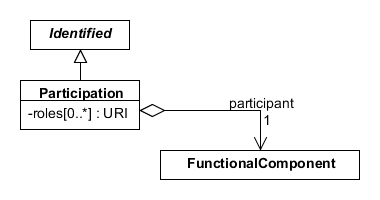
\includegraphics[scale=0.6]{uml/participation}
\caption[]{Diagram of the \sbol{Participation} class and its associated properties.}
\label{uml:participation}
\end{center}
\end{figure}
}

\subsubsection{Participation}
\label{sec:Participation}

Each \sbol{Participation} represents how a particular \sbol{FunctionalComponent} behaves in its parent
\sbol{Interaction}.

\paragraph{The \sbolheading{roles} property}\label{sec:roles:P}

\twozeroone{The \sbolmult{roles:P}{roles} property is a REQUIRED set of \sbol{URI}s that describes the behavior of a \sbol{Participation} (and by extension its referenced \sbol{FunctionalComponent}) in the context of its parent \sbol{Interaction}.

The \sbolmult{roles:P}{roles} property MUST contain one or more \sbol{URI}s that MUST identify terms from appropriate ontologies. It is RECOMMENDED that exactly one \sbol{URI} contained by the \sbolmult{roles:P}{roles} property refer to a term from the participant role branch of the SBO.} \ref{tbl:participant_roles} provides a list of possible SBO terms for the \sbolmult{roles:P}{roles} property and their corresponding \sbol{URI}s.

\begin{table}[ht]
  \begin{edtable}{tabular}{lll}
    \toprule
    \textbf{Participation Role} & \textbf{URI for SBO Term} & \textbf{Interaction Types}\\
    \midrule
    Inhibitor  & \url{http://identifiers.org/biomodels.sbo/SBO:0000020} & Inhibition\\
    Inhibited  & \url{http://identifiers.org/biomodels.sbo/SBO:0000642} & Inhibition\\
    Stimulator & \url{http://identifiers.org/biomodels.sbo/SBO:0000459}  & Stimulation\\
    Stimulated & \url{http://identifiers.org/biomodels.sbo/SBO:0000643}  & Stimulation\\
     Reactant & \url{http://identifiers.org/biomodels.sbo/SBO:0000010}  & Non-Covalent Binding, Degradation \\
     & & Biochemical Reaction \\
    Product & \url{http://identifiers.org/biomodels.sbo/SBO:0000011}  & Non-Covalent Binding, Genetic Production, \\
    & & Biochemical Reaction\\
    Promoter  & \url{http://identifiers.org/biomodels.sbo/SBO:0000598} & Inhibition, Stimulation, Genetic Production\\
    Modifier  & \url{http://identifiers.org/biomodels.sbo/SBO:0000019} & Biochemical Reaction\\
    Modified  & \url{http://identifiers.org/biomodels.sbo/SBO:0000644} & Biochemical Reaction\\
    Control  & \url{http://identifiers.org/biomodels.sbo/SBO:0000168} & Control\\
    Template  & \url{http://identifiers.org/biomodels.sbo/SBO:0000645} & Genetic Production\\
%    Ligand & \url{http://identifiers.org/biomodels.sbo/SBO:0000280}\\
%    Non-Covalent Complex & \url{http://identifiers.org/biomodels.sbo/SBO:0000253}\\
    \bottomrule
  \end{edtable}
  \caption{SBO terms to specify the \sbolmult{roles:P}{roles} property of a \sbol{Participation}.}
  \label{tbl:participant_roles}
\end{table}

If a \sbol{Participation} is well described by one of the terms from \ref{tbl:participant_roles}, then its \sbolmult{roles:P}{roles} property MUST contain the \sbol{URI} that identifies this term.
\twozeroone{Also, if a \sbol{Participation} belongs to an \sbol{Interaction} that has a type listed in \ref{tbl:interaction_types}, then the \sbol{Participation} SHOULD have a role that is cross-listed with this type in \ref{tbl:participant_roles}.}
Lastly, if the \sbolmult{roles:P}{roles} property of a \sbol{Participation} contains multiple
 \sbol{URI}s, then they MUST identify non-conflicting terms. For example, the SBO terms ``stimulator'' and ``inhibitor'' would conflict.


\paragraph{The \sbolheading{participant} property}\label{sec:participant}

The \sbol{participant} property MUST specify precisely one \sbol{FunctionalComponent} object that plays the designated role in its parent \sbol{Interaction} object.


\paragraph{Serialization}

The serialization of \sbol{Participation} objects has the following form.
\lstsetsbol
\begin{lstlisting}
<sbol:Participation rdf:about="...">
  ... [\emph{properties inherited from identified}] ...
  [\emph{zero or more}] <sbol:role rdf:resource="..."/> [\emph{elements}]
  [\emph{one}]          <sbol:participant rdf:resource="..."/> [\emph{element}]
</sbol:Participation>
\end{lstlisting}

In the example below, the role of participating \sbol{FunctionalComponent} is defined to be \external{inhibitor}, using the \external{SBO:0000020} term. This component is specified using the \sbol{participant} property of the \sbol{Participation} entity.
\lstsetsbol
\begin{lstlisting}
<sbol:Participation rdf:about="http://sbolstandard.org/example/laci_inverter/LacI_pLacI/P03023">
  <sbol:role rdf:resource="http://identifiers.org/biomodels.sbo/SBO:0000020"/>
  <sbol:participant rdf:resource="http://sbolstandard.org/example/laci_inverter/TF"/>
</sbol:Participation>
\end{lstlisting}

\subsection {Collection}
\label{sec:Collection}
The \sbol{Collection} class is a class that groups together a set of \sbol{TopLevel} objects that have something in common.
Some examples of \sbol{Collection} objects:
\begin{itemize}
\item Results of a query to find all \sbol{ComponentDefinition} objects in a repository that function as promoters.
\item A set of \sbol{ModuleDefinition} objects representing a library of genetic logic gates.
\item A \sbol{ModuleDefinition} for a complex design, and all of the \sbol{ModuleDefinition}, \sbol{ComponentDefinition}, \sbol{Sequence}, and \sbol{Model} objects used to provide its full specification.
\end{itemize}

\begin{figure}[ht]
\begin{center}
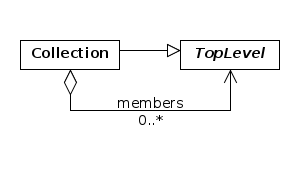
\includegraphics[scale=0.6]{uml/collection}
\caption[]{Diagram of the \sbol{Collection} class and its associated properties.}
\label{uml:collection}
\end{center}
\end{figure}

\subsubsection*{The \sbolheading{members} property}\label{sec:members}
The \sbol{members} property of a \sbol{Collection} is OPTIONAL and MAY contain a set of \sbol{URI} references to zero or more \sbol{TopLevel} objects.

\subsubsection*{Serialization}

The serialization of a \sbol{Collection} has the following form:

\lstsetsbol
\begin{lstlisting}
<sbol:Collection rdf:about="...">
  ... [\emph{properties inherited from identified}] ...
  [\emph{zero or more}] <sbol:member rdf:resource="..."/> [\emph{element}]
</sbol:Collection>
\end{lstlisting}

The example below shows the serialization of a \sbol{Collection} object grouping together a library of constitutive promoters.
\lstsetsbol
\begin{lstlisting}
<?xml version="1.0" ?>
<rdf:RDF xmlns:rdf="http://www.w3.org/1999/02/22-rdf-syntax-ns#" xmlns:dcterms="http://purl.org/dc/terms/" xmlns:prov="http://www.w3.org/ns/prov#" xmlns:sbol="http://sbols.org/v2#">
  <sbol:Collection rdf:about="http://parts.igem.org/Promoters/Catalog/Anderson">
    <sbol:persistentIdentity rdf:resource="http://parts.igem.org/Promoters/Catalog/Anderson"/>
    <sbol:displayId>Anderson</sbol:displayId>
    <dcterms:title>Anderson promoters</dcterms:title>
    <dcterms:description>The Anderson promoter collection</dcterms:description>
    <sbol:member rdf:resource="http://partsregistry.org/Part:BBa_J23119"/>
    ...
    <sbol:member rdf:resource="http://partsregistry.org/Part:BBa_J23118"/>
  </sbol:Collection>
</rdf:RDF>
\end{lstlisting}
\label{ser:Collection}

\subsection{Annotation and Extension of SBOL}
\label{sec:Annotations}

SBOL does not currently represent all types of biological design data, since many of these data types (e.g., biological context and design performance metrics) lack a clear consensus on their proper representation. In addition, some types of biological data are not directly relevant to design and are therefore outside of the scope of SBOL.

To enable representation of these data, SBOL allows developers to embed custom data within SBOL objects and documents, such that these data can be exchanged without being damaged or lost. This annotation and extension mechanism is designed to enable new types of data to be easily incorporated into the SBOL standard once there is community consensus on their proper representation.

Several methods are supported for connecting the SBOL data model with other types of application-specific data:
\begin{itemize}
\item Custom data can be added to an SBOL object by annotating that object with non-conflicting properties. These properties could contain \sbol{literal} data types such as \sbol{String}s or \sbol{URI}s that require a resolution mechanism to obtain external data. An example is annotating a \sbol{ComponentDefinition} with  a property that contains a \sbol{String} description and \sbol{URI} for the parts registry from which its source data was originally imported.
\item Custom data in the form of independent objects can be added to an SBOL document by  creating \sbol{GenericTopLevel} objects and annotating them as described above. An example is a \sbol{GenericTopLevel} object that is annotated such that it represents a data sheet that describes the performance of a \sbol{ModuleDefinition} in a particular context.
\item Finally, just as custom objects can be embedded in an  SBOL document, external documents can embed or refer to SBOL objects. Support for this last case is not explicitly provided in this specification. Rather, this case depends on the external non-SBOL system managing its relationship to SBOL and data serialized in RDF/XML, and is included here for completeness.
\end{itemize}

\subsubsection{Annotating SBOL objects}
% whole set of labels for the properties defined herein
\label{sec:qName}
\label{sec:QName}
\label{sec:value}
\label{sec:Annotation}
\label{sec:AnnotationValue}
\label{sec:NestedAnnotations}
\label{sec:nestedQName}
\label{sec:nestedURI}

Each \sbol{Identified} object MAY contain any number of \sbol{Annotation} objects that store data in the form of name/value property pairs. The \sbol{qName} is REQUIRED and MUST contain a \sbol{QName}, which is composed of a namespace, an OPTIONAL prefix, and a local name. The \sbol{qName} property MUST be stored in the data model to allow for proper serialization as described below.
The \sbol{value} property is also REQUIRED and MUST contain a \sbol{literal} (i.e., a \sbol{String}, \sbol{Integer}, \sbol{Double}, \sbol{Boolean}), \sbol{URI}, or \sbol{NestedAnnotations} object. A \sbol{NestedAnnotations} object MUST contain \sbol{nestedQName} and \sbol{nestedURI} properties, and it MAY contain an \sbol{annotations} property that contains zero or more \sbol{Annotation} objects.

\begin{figure}[!ht]
\begin{center}
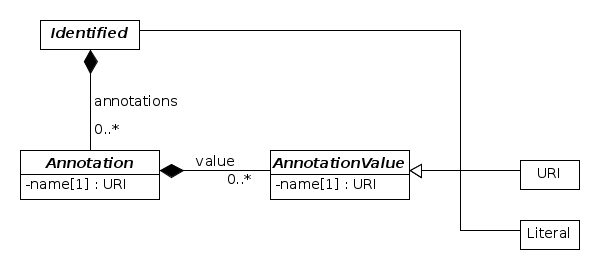
\includegraphics[scale=0.55]{uml/identified_annotations}
\caption[]{Diagram of the \sbol{Annotation} class and its association with \sbol{Identified} and \sbol{AnnotationValue} objects, which is used for annotating SBOL entities with application specific data.}
\label{uml:identified_annotations}
\end{center}
\end{figure}

\subsubsection*{Serialization}

The serialization of an \sbol{Annotation} has the following form:

\lstsetsbol
\begin{lstlisting}
<?xml version="1.0" ?>
<rdf:RDF xmlns:rdf="http://www.w3.org/1999/02/22-rdf-syntax-ns#"
  xmlns:sbol="http://sbols.org/v2#"
  xmlns:prefix1="NAMESPACE_1"
  xmlns:prefix2="NAMESPACE_2"
  xmlns:nestedObjectPrefix="A_NESTED_OBJECT_NAMESPACE"
  ...
 >
<sbol:A_TOPLEVELOBJECT rdf:about="...">
                ...
  [\emph{zero or more}] <prefix1:LOCAL_NAME_1>A_LITERAL</prefix1:LOCAL_NAME_1> [\emph{elements}]
  [\emph{zero or more}] <prefix1:LOCAL_NAME_2 rdf:resource=URI/> [\emph{elements}]
  [\emph{zero or more}] <prefix2:LOCAL_NAME_3>
                  <nestedObjectPrefix:NESTED_LOCAL_NAME rdf:about="...">
                    ...
                  </nestedObjectPrefix:NESTED_LOCAL_NAME>
                </prefix2:LOCAL_NAME_3> [\emph{elements}]
</sbol:TOPLEVELOBJECT>
\end{lstlisting}
The \sbol{qName} property specifies a namespace, prefix, and local part/name. The use of such qualified names is described in detail by the W3C (\url{http://www.w3.org/TR/1999/REC-xml-names-19990114/#ns-using}). Essentially, the "xmlns" property defines the prefix \sbol{String} to use as an alias for the namespace.  The prefix can be any \sbol{String}. Its use is OPTIONAL, since it simply replaces the full namespace, thereby making the serialization easier for a human to read.

The first form of \sbol{Annotation} shown above is for an \sbol{Annotation} that contains a \sbol{literal} as its \sbol{value}. The second form is for an  \sbol{Annotation} that contains a \sbol{URI} as its value. Finally, the third form is for an \sbol{Annotation} that contains a  \sbol{NestedAnnotations} object as its value. In the last case, the \sbol{nestedQName} property specifies the nested namespace, nested prefix, and nested local part/name, while the \sbol{nestedURI} property species the \sbol{URI} for the \sbol{NestedAnnotations} object.

The example below shows how the serialization for a promoter \sbol{ComponentDefinition} can be annotated with custom data. \sbol{Annotation}s are added containing the relevant information from the iGEM Parts Registry. Each property serialization of an \sbol{Annotation} is qualified with the \external{http://www.partsregistry.org/} namespace, which is prefixed using \external{pr}. The first \sbol{Annotation} is named \external{pr:group}. It specifies the iGEM group that has designed the promoter and has a \sbol{String} value.
The second \sbol{Annotation} is named \external{pr:experience}. It contains a \sbol{URI} value that is serialized as an RDF resource and can be resolved to the information Web page on the Parts Registry for the promoter.
Finally, the third \sbol{Annotation} is named \external{pr:information}. It contains a \sbol{NestedAnnotations} object that is serialized as shown and includes information about the regulatory details of the promoter using \sbol{Annotations} that correspond to Parts Registry categories.

\begin{figure} [ht]
\lstsetsbol
\begin{lstlisting}
<?xml version="1.0" ?>
<rdf:RDF xmlns:pr="http://partsregistry.org" xmlns:rdf="http://www.w3.org/1999/02/22-rdf-syntax-ns#" xmlns:dcterms="http://purl.org/dc/terms/" xmlns:prov="http://www.w3.org/ns/prov#" xmlns:sbol="http://sbols.org/v2#">
  <sbol:ComponentDefinition rdf:about="http://partsregistry.org/cd/BBa_J23119">
    <sbol:persistentIdentity rdf:resource="http://partsregistry.org/cd/BBa_J23119"/>
    <sbol:displayId>BBa_J23119</sbol:displayId>
    <pr:group>iGEM2006_Berkeley</pr:group>
    <pr:experience rdf:resource="http://parts.igem.org/cgi/partsdb/part_info.cgi?part_name=BBa_J23119"/>
    <pr:information>
      <pr:Information rdf:about="http://parts.igem.org/cgi/partsdb/part_info.cgi?part_name=BBa_J23119">
        <pr:sigmafactor>//rnap/prokaryote/ecoli/sigma70</pr:sigmafactor>
        <pr:regulation>//regulation/constitutive</pr:regulation>
      </pr:Information>
    </pr:information>
    <dcterms:title>J23119</dcterms:title>
    <dcterms:description>Constitutive promoter</dcterms:description>
    <sbol:type rdf:resource="http://www.biopax.org/release/biopax-level3.owl#DnaRegion"/>
    <sbol:role rdf:resource="http://identifiers.org/so/SO:0000167"/>
  </sbol:ComponentDefinition>
</rdf:RDF>
\end{lstlisting}
\label{ser:Annotation}
\end{figure}

\subsubsection{GenericTopLevel}
\label{sec:GenericTopLevel}
\label{sec:rdfType}

Custom data can also be embedded at the top level of an SBOL document. The \sbol{GenericTopLevel} class is used to represent top-level entities whose purpose is to contain a set of annotations that are independent of any other class of SBOL object.
Entities that have independent existence and are not recognized by the SBOL standard are deserialized to \sbol{GenericTopLevel} objects.
These \sbol{GenericTopLevel} objects can be safely used by tools to exchange non-SBOL data.

As with other \sbol{TopLevel} objects, \sbol{GenericTopLevel} objects MAY include the properties \sbol{displayId}, \sbol{name}, \sbol{description}, etc. The type of data annotating a \sbol{GenericTopLevel} object is indicated using the REQUIRED \sbol{rdfType} property, which MUST contain a \sbol{QName}. As before with the \sbol{qName} property, the \sbol{rdfType} property is used to set the namespace, prefix, and local part/name during serialization.

\begin{figure}[ht]
\begin{center}
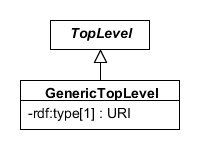
\includegraphics[scale=0.6]{uml/generictoplevel}
\caption[]{Diagram of the \sbol{GenericTopLevel} class and its associated properties, which is used for embedding externally defined entities into SBOL documents.}
\label{uml:generictoplevel}
\end{center}
\end{figure}

\subsubsection*{Serialization}

The serialization of the \sbol{GenericTopLevel} class has the following form, where the prefix, namespace, and local part/name are defined by the \sbol{rdfType} property:

%<?xml version="1.0" ?>
%<rdf:RDF ... xmlns:prefix=namespace ...>
%<prefix:localPart rdf:about="...">
%              ...
%</prefix:localPart>

\lstsetsbol
\begin{lstlisting}
<?xml version="1.0" ?>
<rdf:RDF xmlns:rdf="http://www.w3.org/1999/02/22-rdf-syntax-ns#"
  xmlns:sbol="http://sbols.org/v2#"
  xmlns:applicationPrefix="APPLICATION_NAMESPACE"
  ...
 >
<applicationPrefix:APPLICATION_OBJECT_NAME rdf:about="...">
  ... [\emph{properties inherited from identified}] ...
  ... [\emph{any non-conflicting application-specific properties}] ...
</applicationPrefix:APPLICATION_OBJECT_NAME>
\end{lstlisting}

The example below shows how a datasheet object can be added to an SBOL document using the \sbol{GenericTopLevel} class.
The J23119 promoter \sbol{ComponentDefinition} is annotated with the \external{myapp:datasheet} property that contains the \sbol{URI} of a \sbol{TopLevel} Datasheet object. The Datasheet object is further annotated with the transcription rate and \sbol{URI} for the actual characterization data using the \external{myapp:transcriptionRate} and \external{myapp:characterizationData} properties, respectively. As specified by their \sbol{rdfType} and \sbol{qName} properties, the \sbol{TopLevel} Datasheet object and all \sbol{Annotation} objects in this example are serialized with the custom \external{\path{http://www.myapp.org/}} namespace and \external{myapp} prefix.

\begin{figure}[ht]
\lstsetsbol
\begin{lstlisting}
<?xml version="1.0" ?>
<rdf:RDF xmlns:myapp="http://www.myapp.org/" xmlns:rdf="http://www.w3.org/1999/02/22-rdf-syntax-ns#" xmlns:dcterms="http://purl.org/dc/terms/" xmlns:prov="http://www.w3.org/ns/prov#" xmlns:sbol="http://sbols.org/v2#">
  <sbol:ComponentDefinition rdf:about="http://www.partsregistry.org/cd/BBa_J23119">
    <sbol:persistentIdentity rdf:resource="http://www.partsregistry.org/cd/BBa_J23119"/>
    <sbol:displayId>BBa_J23119</sbol:displayId>
    <prov:wasDerivedFrom rdf:resource="http://www.partsregistry.org/Part:BBa_J23119"/>
    <myapp:datasheet rdf:resource="http://www.partsregistry.org/gen/datasheet1"/>
    <dcterms:title>J23119</dcterms:title>
    <dcterms:description>Constitutive promoter</dcterms:description>
    <sbol:type rdf:resource="http://www.biopax.org/release/biopax-level3.owl#DnaRegion"/>
    <sbol:role rdf:resource="http://identifiers.org/so/SO:0000167"/>
  </sbol:ComponentDefinition>
  <myapp:Datasheet rdf:about="http://www.partsregistry.org/gen/datasheet1">
    <sbol:persistentIdentity rdf:resource="http://www.partsregistry.org/gen/datasheet1"/>
    <sbol:displayId>datasheet1</sbol:displayId>
    <myapp:characterizationData rdf:resource="http://www.myapp.org/measurement/1"/>
    <myapp:transcriptionRate>1</myapp:transcriptionRate>
    <dcterms:title>Datasheet 1</dcterms:title>
  </myapp:Datasheet>
</rdf:RDF>
\end{lstlisting}
\label{ser:GenericTopLevel}
\end{figure}

\section{Mapping Between SBOL 1.1 and SBOL 2.0}
\label{sec:mapping}

\ref{SBOL1TO2} depicts the mapping of SBOL 1.1 classes to SBOL 2.0 classes, indicating corresponding classes/properties by color.
The SBOL 2.0 \sbol{Model} and \sbol{ModuleDefinition} classes have no SBOL 1.1 equivalent, and thus are not shown.
In particular:
\begin{itemize}
\item SBOL 1.1 \external{Collection} objects containing \external{DnaComponent} objects map to SBOL 2.0 \sbol{Collection} objects that contain \sbol{ComponentDefinition} objects with DNA \sbolmult{types:CD}{types} properties.
\item SBOL 1.1 \external{DnaComponent} objects maps to SBOL 2.0 \sbol{ComponentDefinition} objects with DNA \sbolmult{types:CD}{types} properties.
\item SBOL 1.1 \external{DnaSequence} objects maps to an SBOL 2.0 \sbol{Sequence} objects with \external{IUPAC DNA} \sbol{encoding} properties.
\item SBOL 1.1 \external{SequenceAnnotation} objects with \external{bioStart} and \external{bioEnd} properties map to SBOL 2.0 \sbol{SequenceAnnotation} objects that contain \sbol{Range} objects.
\item SBOL 1.1 \external{SequenceAnnotation} objects that lack \external{bioStart} and \external{bioEnd} properties map to an SBOL 2.0 \sbol{SequenceAnnotation} objects that contain \sbol{GenericLocation} objects.
\item Each SBOL 1.1 \external{SequenceAnnotation} also maps to an SBOL 2.0 \sbol{Component}, which represents the instantiation or usage of the appropriate \sbol{ComponentDefinition}.
\item Each SBOL 1.1 \external{precedes} property maps to an SBOL 2.0 \sbol{SequenceConstraint} that specifies a precedes \sbol{restriction} property.
\end{itemize}

\begin{figure*}[h]
\begin{center}
  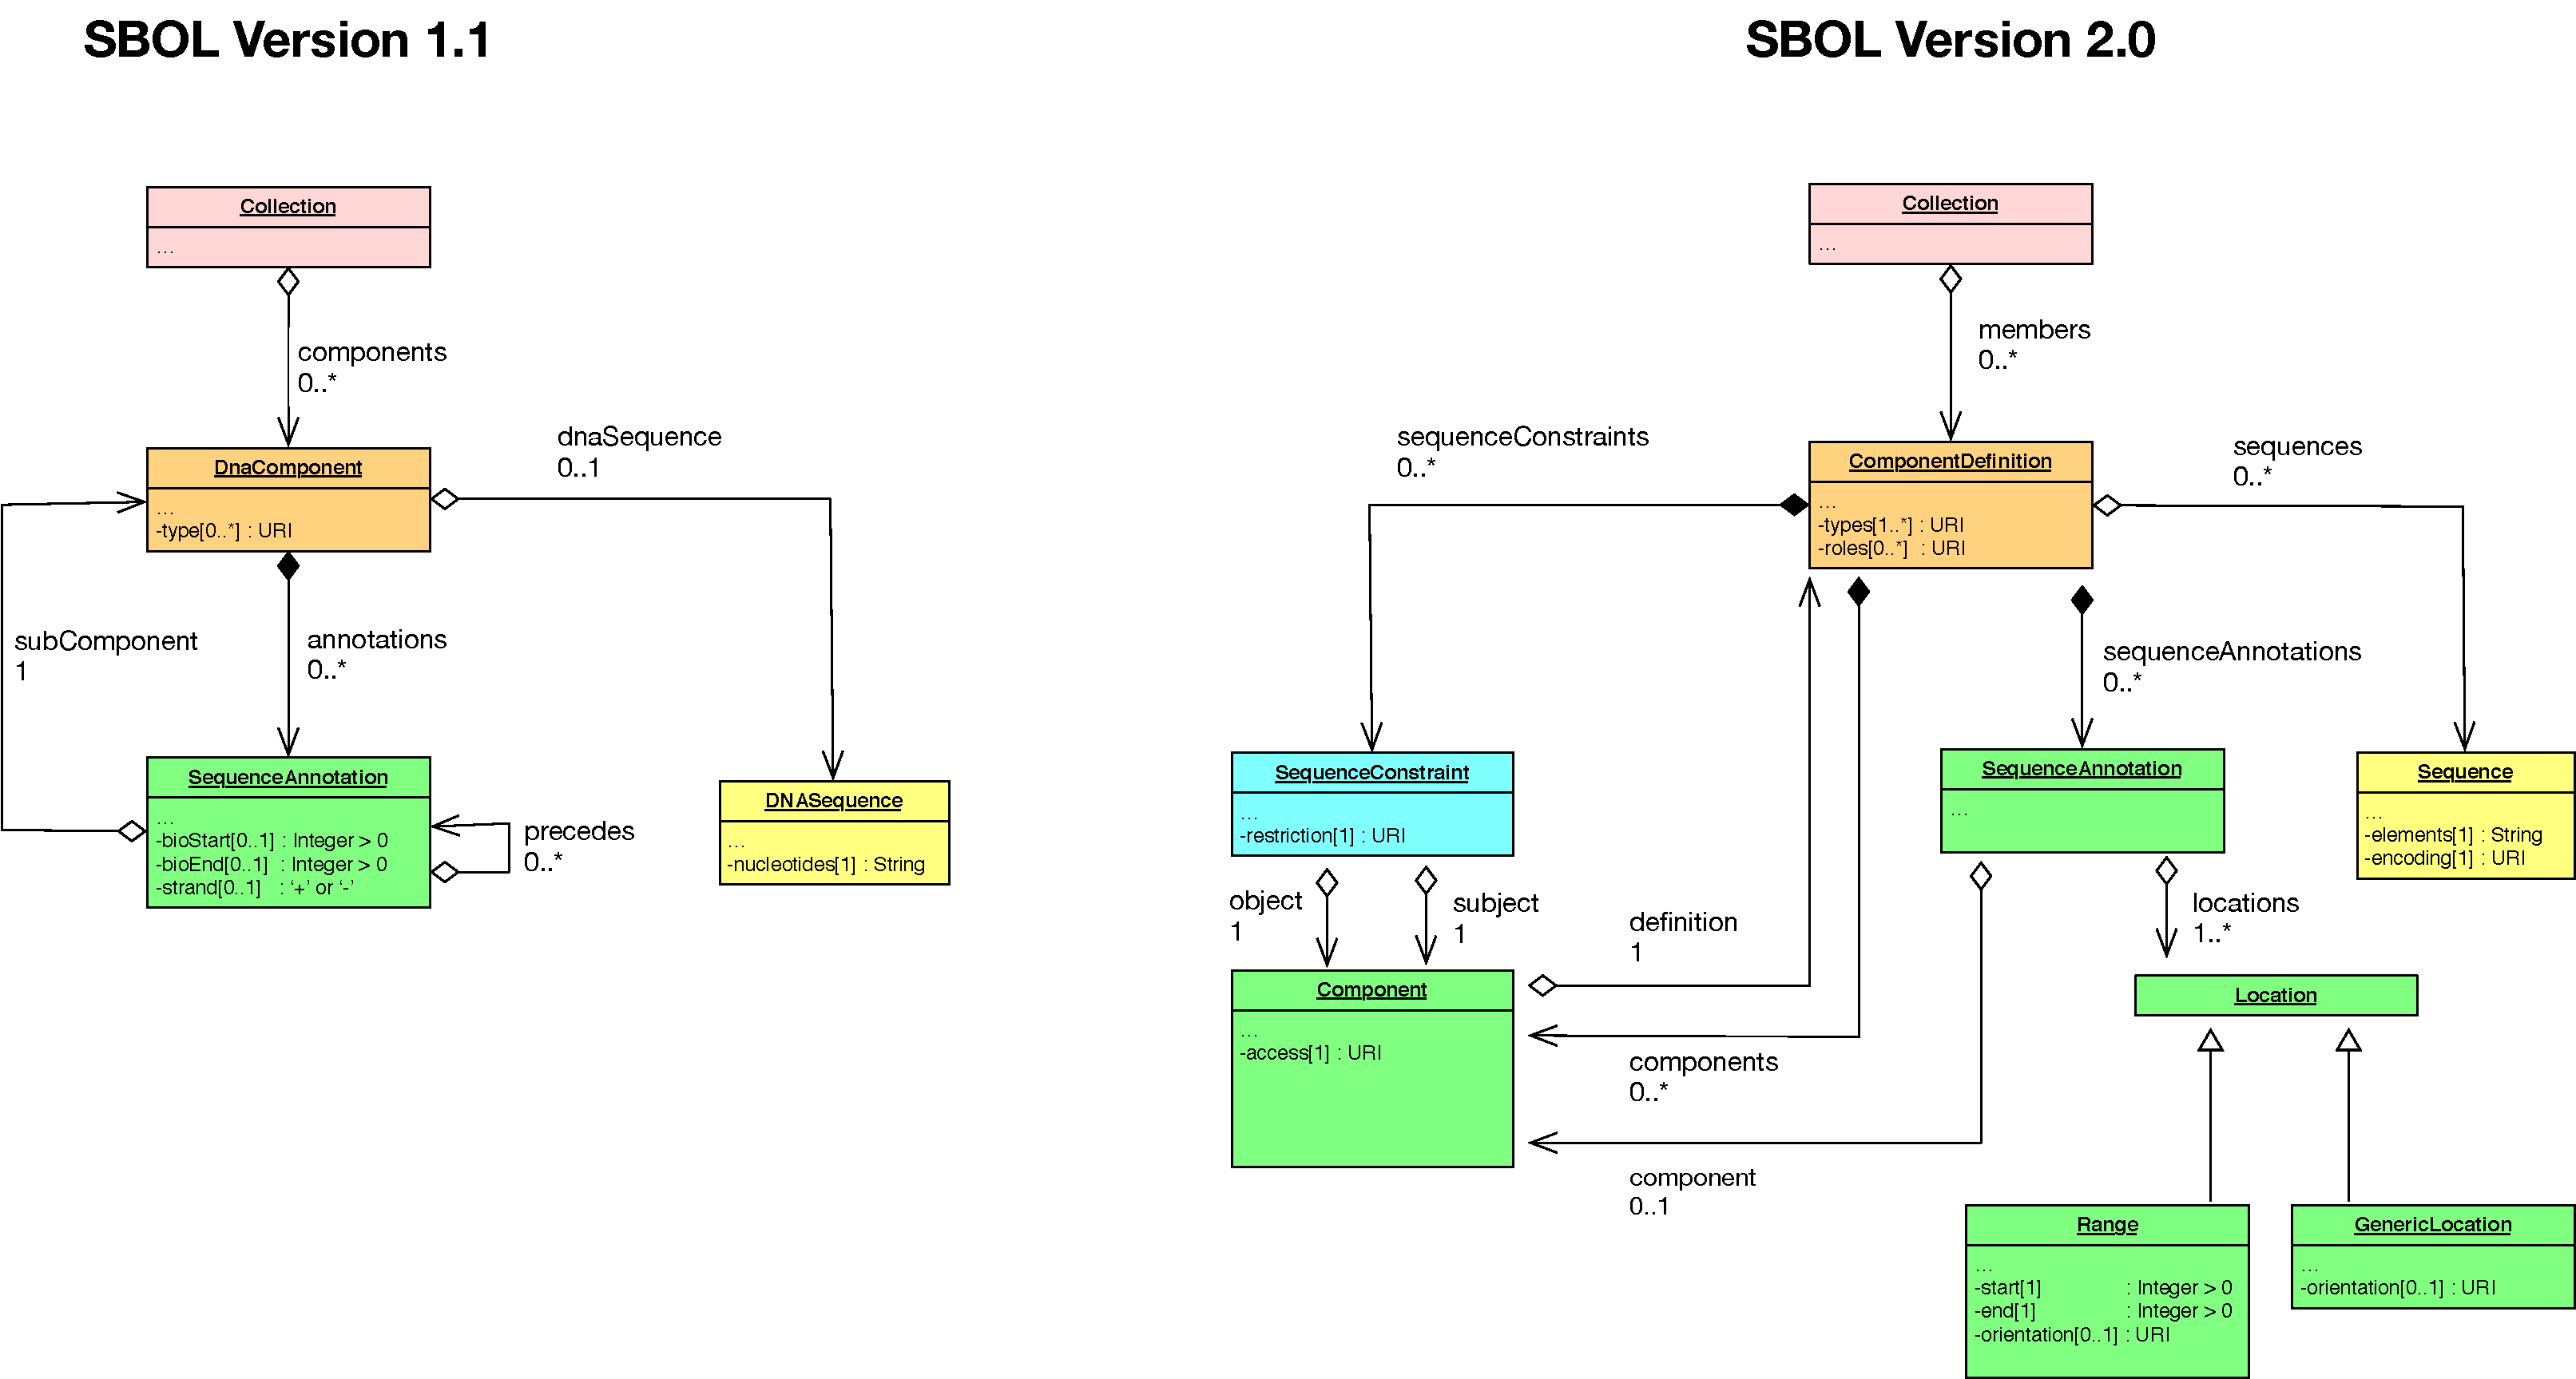
\includegraphics[width=\textwidth]{images/sbol_v1_to_v2}
\end{center}
\caption{\label{SBOL1TO2}The mapping from the SBOL 1.1 data model to the SBOL 2.0  data model, indicating corresponding classes/properties by color.}
\end{figure*}
